\documentclass[a4paper,12pt]{report}
\usepackage{graphicx}
\title{Resume Database}
\author{Nuha Hanifatul Khonsa'}
\date{17 oktober 2019}
\begin{document}


\maketitle

\chapter{}
\section{Agenda}
\begin{enumerate}
    \item Pengembangan Aplikasi Kode Rendah
    \item Aplikasi Orecle Express: Ikhtisar
    \item Mengonversi Spreadsheet Ke Aplikasi Web Dalam Hitungan Menit- Demo Aplikasi
    \item Oracle Mengungkapkan Fitur Produk Dan Demo
    \item Orecle Apex: Pendidikan
    \item Laboratorium Tangan
\end{enumerate}

\section{Apa itu Kode Rendah?}
\begin{enumerate}
    \item Mudah dijalankan
    \item Sangat produktif
    \item Dapat diperpanjang
    \item Scalable
    \item Fungsionalitas : Dengan kode yang lebih sedikit 
\end{enumerate}

\section{What is Orecle Apex}
\textit{Platform pengembangan kode-rendah  yang memungkinkan untuk membangun skalabilitas dan aman . Sebagai aplikasi perusahaan kelas dunia dengan fitur yang dapat digunakan dimana saja.}

\section{Pengembangan Aplikasi pada Perusahaan}
\begin{enumerate}
    \item Membutuhkan Sumber Daya Pengembangan Khusus Dan Mahal
    \item Panjang Siklus Dev Aplikasi
    \item Backlog Yang Besar
    \item Kolaborasi Minimal
    \item Bisnis Menyelesaikan Masalah Dengan Alat Yang Salah
\end{enumerate}

\section{Orecle APEX Pengembangan Aplikasi Data Rendah Pertama}
\begin{center}
    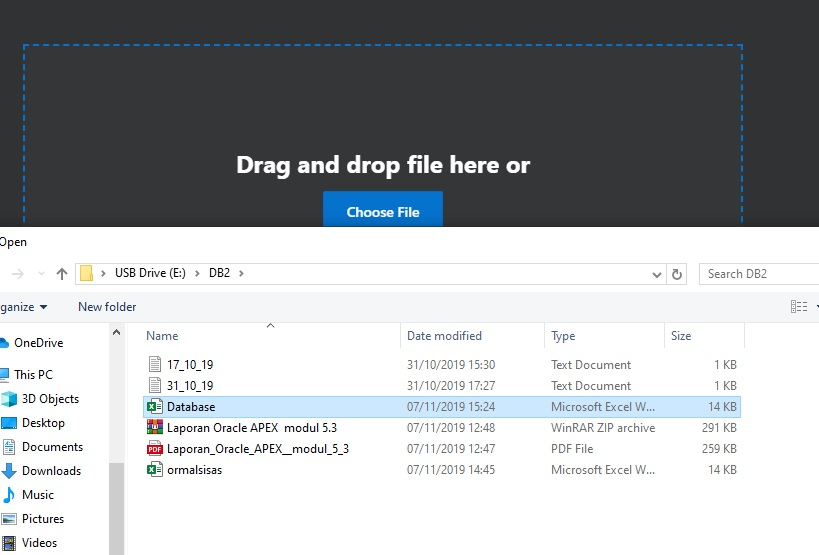
\includegraphics[width=11cm\textwidth]{2.jpg}
\end{center}

\section{Mengelola Data Dalam Spreadsheet Menantang}
\begin{enumerate}
    \item Memvalidasi Data Secara Manual Dan Rawan Kesalahan
    \item Integritas Data -Tidak Dapat Menjamin Keakuratan Data pada Lingkungan Multi-Pengguna.
    \item Keamanan Data Tidak Efektif
    \item Berbagi Data-Excel Lamban Dan Sulit Untuk Dibagikan
\end{enumerate}

\section{
Jenis Aplikasi Apa Yang Cocok Untuk Oracle Apex?}
\begin{enumerate}
    \item Large mission-critical apps for thousand of users
    \item Fill in gaps in corporate systems
    \item Steamline outed business processes
    \item Modernization of legacy systems
    \item Self-service apps for all employees
    \item Customer/Partner-facing portals
    \item proof of concepts
    \item Quick =-win apps (lifespan < a few months
    \item Replacing spreadsheets
\end{enumerate}

\section{Apa Itu Oracle Apex?}
\textbf Kerangka kerja pengembangan aplikasi web database-centric.
\begin{center}
    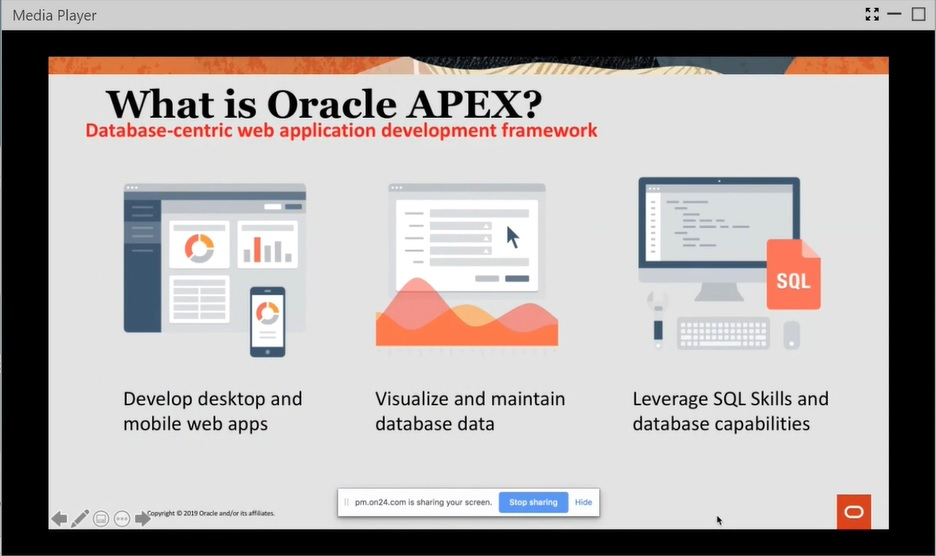
\includegraphics[width=11cm\textwidth]{apa.jpg}
\end{center}
\begin{enumerate}
    \item Mengembangkan Aplikasi Web Desktop Dan Seluler, 
    \item Memvisualisasikan Dan Memelihara Data Basis Data, 
    \item Meningkatkan Keterampilan Sql Dan Kemampuan Basis Data.
\end{enumerate}

\section{Oracle Apex: Use Cases}
\subsection{Memodernisasi Formulir Orecle }
\textbf Fitur
\begin{enumerate}
    \item Seret daan letakkan file Xls, Csv, Xml, Atau Json
    \item Membuat tabel dalam Database Autonomous
    \item Unggah aplikasi ke tabel baru
    \item Buat Aplikasi Berdasarkan Tabel Baru Solusi 
\end{enumerate}
\textbf Solusi
\begin{enumerate}
    \item Sumber kebeneran tunggal
    \item Kirim URL bukan file
    \item Aplikasi yang aman, terukur, multi pengguna
    \item Perluasan dengan bagan, kalender, validasi, dan lainnya
\end{enumerate}
\subsection{Pengembangan Aplikasi yang Cepat} 
\textbf{Fitur}
\begin{enumerate}
    \item Membangun aplikasi dalam beberapa hari / minggu bukan bulan / tahun
    \item Gunakan penyihir yang kuat untuk membuat aplikasi berfitur lengkap
    \item Mudah dimodifikasi untuk memenuhi perubahan persyaratan
    \item Dengan cepat beralih ke aplikasi yang siap produksi
    \item Kemampuan kode rendah memungkinkan profesional non-IT juga membangun atau membantu membangun aplikasi
\end{enumerate}
\textbf{Solusi}
\begin{enumerate}
    \item Oportunistik
    \item Aplikasi taktis sederhana untuk memenuhi kebutuhan mendesak
    \item Webify proses kertas
    \item Umumnya dikembangkan oleh satu atau dua orang
\end{enumerate}
\subsection{Memperluas Sistem Perusahaan}
\textbf{Fitur}
\begin{enumerate}
    \item Perluas ERP dan perangkat lunak perusahaan lainnya
    \item Menyediakan dasbor khusus organisasi
    \item Alur kerja yang ditingkatkan
    \item Isi celah
\end{enumerate}
\textbf{Solusi}
\begin{enumerate}
    \item Memenuhi persyaratan non-standar
    \item Optimalkan fungsi bisnis umum
    \item Tingkatkan pengambilan data
    \item Mengintegrasikan sumber data yang berbeda
\end{enumerate}
\section{Orecle APEX: Distinguishing Characteristic}
\textit {Pengembangan Aplikasi  IDE adalah browser web. Tidak perlu perangkat lunak klien. Aplikasi disimpan pada Database sebagai data meta. Deklaratif – didak ada pembuatan kode, Halaman efisien hanya ada 1 request dan  1 respon pemrosesan data dilakukan dalam database}.
\section{Fitur Tanpa Biaya dari Database Orecle}
\subsection{Fitur yang didukung penuh tanpa biaya}
\begin{enumerate}
    \item Beberapa Aplikasi, Pengembang dan Pengguna Akhir
    \item Tim Dukungan Oracle Khusus
    \item 11gr2, 12c, 18c
    \item Semua Edisi DB EE, SE2, XE , 
\end{enumerate}
\subsection{Termasuk Dengan Layanan Clound Oracle}
\begin{unumerate}
    \item Database Mandiri 
    \item Database Sebagai Layanan
    \item Tidak Ada Evaluasi Biaya http: //Apex.Oracle.Com
\end{unumerate}
\subsection{Mudah untuk Diinstal}
\begin{enumerate}
    \item Termasuk secara default dengan semua edisi database Orecle
    \item Unduh Formuli terbaru http://apex.orecle.com/otp
\end{enumerate}

\section{Opsi Opsi Deveploment / Penyebaran}
\subsection{Lokal}
\begin{enumerate}
    \item 	Instal Pada Laptop Yang Berdiri Sendiri Menggunakan Edisi Oracle Express Edition (Xe) Atau Database Lengkap.
    \item Cukup Tingkatkan Apex Ke Versi Yang Diperlukan.
    \item Dapat Bekerja Sepenuhnya Tanpa Terputus.
\end{enumerate}
\subsection{Di Tempat}
\begin{enumerate}
    \item Biasanya Dijalankan Oleh Departemen TI
    \item TI Umumnya Adalah Layanan Operasi Produksi, Dan Penyedia Layanan
    \item Departemen Yang Bertanggung Jawab Untuk Pengembangan Aplikasi.
    \item Fitur Tanpa Biaya Dari Database Oracle
\end{enumerate}
\subsection{Cloud}
\begin{enumerate}
    \item Menyebarkan aplikasi internet
    \item  Dihapus untuk pengembangan aplikasi yang cepat, penerimaan pengguna dan pelatihan
    \item Prototyping dan Proof-of-Concept
    \item Perusahaan konsultan mengembangkan untuk penempatan premis pelanggan
\end{enumerate}

\section{Mesin Virtual Basis Data Tunggal / Beberapa Ruang Kerja}
\begin{center}
    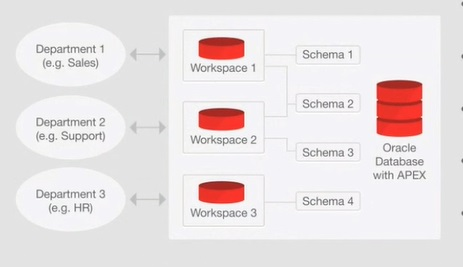
\includegraphics[width=11cm\textwidth]{ruang.jpg}
\end{center}
\begin{enumerate}
    \item Ruang kerja yang digunakan untuk mendefinisikan definisi aplikasi / Skema menyimpan data
    \item Hubungan Banyak-ke-banyak antara Ruang Kerja dan Skema
    \item Instance Administrator mengelola lingkungan dan akses skema
    \item Departemen dapat meminta lebih banyak ruang, dan akses ke skema baru
    \item Misalnya, layanan hanya-internal Oracle http://apex.oraclecorp.com memiliki lebih dari 5.000 Workspaces, yang mencakup setiap lini bisnis di Oracle
\end{enumerate}
\section{Community}
\begin{center}
    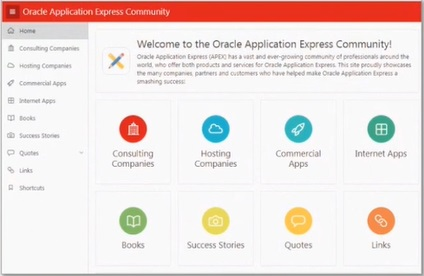
\includegraphics[width=11cm\textwidth]{Community.jpg}
\end{center}
\begin{enumerate}
    \item Lebih dari 500,00 pengembang di seluruh dunia
    \item Diperkirakan dari permintaan dukungan, unduhan, konferensi, aktivitas forum diskusi
    \item Lebih dari 100 blogger aktif http: //odtug.com/apex
    \item http://apex.oralce.com/komunitas konsultasi masyarakat, buku, kesuksesan, cerita, kutipan, aplikasi komersial
\end{enumerate}
\section{Pendidikan}
\textit{Jika Anda Seorang Siswa Atau Guru SQL, Database Relasional, atau Pengembangan Aplikasi, Anda Dapat Menggunakan Oracle Apex Untuk dapat Memperkaya Pengalaman Pendidikan Anda}
\section{Sertifikasi Orecle}
\textit{Setelah Anda Mahir dalam pengembangkan Aplikasi APEX, Anda Dapat Mengikuti Ujian Sertifikasi Oracle Menjadi Aplikasi Oracle Express 18 sebagai Profesional Bersertifikat Pengembang.
Dan Buktikan Kepada Semua Orang Bahwa Anda Tahu Cara Membangun Aplikasi Yang Kuat Dengan Menggunakan Apex.}
\section{Kurikulum Orecle Apex}
\begin{enumerate}
    \item Pelajar, Dan Panduan Praktikum Di Laboratorium
    \item Total 16 Pelajaran Dan 15 Tangan Di Laboratorium
    \item PPT, PDF, Sumber, Dan File Lab
    \item Lab / Demo Dapat Dilakukan Pada: Contoh Akademi Oracle
\end{enumerate}
\section{Gambaran Umum}
\textit{Lab Ini Menuntun Anda Saat Mengunggah Spreadsheet Ke Tabel Database Oracle, Lalu Membuat Aplikasi Berdasarkan Tabel Baru Ini.  Anda Kemudian Akan Bermain Dengan Laporan Interaktif Dan Meningkatkan Formulir Terlampir.  Terakhir, Anda Akan Menambahkan Halaman Kalender Dan Kemudian Menautkannya Ke Halaman Formulir Yang Ada.  Alih-Alih Mencoba Mengirim Surel Spreadsheet Untuk Mengumpulkan Informasi Dari Orang Yang Berbeda, Cukup Buat Aplikasi Dalam Hitungan Menit, Dan Kirim Surel URL.  Spreadsheet Sumber-Kebenaran-Tunggal, Multi-Pengguna, Aman, Dan Mudah Tersiram Ini!  Aplikasi Scren Jadi Lebih Baik}

\chapter{}
\section{Memulai Orecle Apex}
\begin{enumerate}
    \item Buka link https://apex.orecle.com
    \item Klik Get Started for Free
    \item Klik Reques a Free Workspace
    \begin{center}
    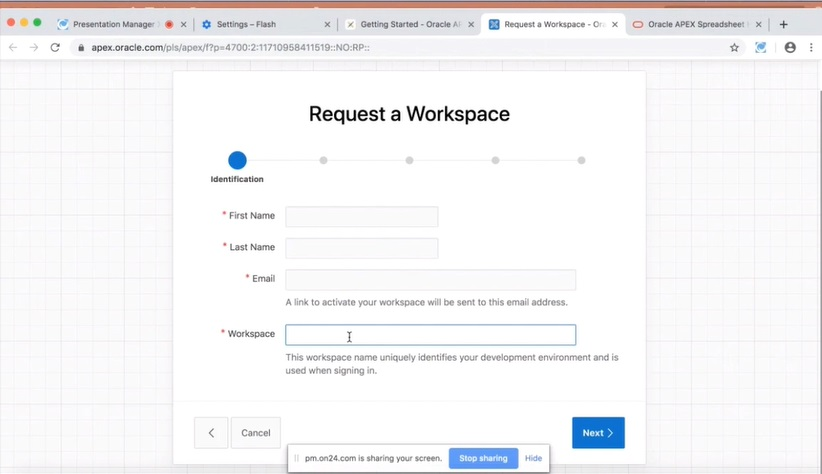
\includegraphics[width=11cm\textwidth]{request.jpg}
    \end{center}
    \item Masukkan data sesuai perintah 
    \item Setelah semua terisi dan klik Next
    \item Cek Email anda.dan buka email dari oracley
    \item Klik Create Workspace
    \item Klik Continue to Log in Screen
    \item Lalu ubah password anda
    \item Dan ikuti semua step yang ada hingga menemui Finis
\end{enumerate}
\textbf{Nb: jika sudah memiliki akun anda dapat melewati Langkah pertama yaitu registrasi oracle apex.}

\Section{Membangun Aplikasi pertama}
\textbf{Membuat Applikasi dari Spreadsheet}
\subsection{Masuk Orecle APEX}
\begin{enumerate}
    \item Masuk Ke Ruang Kerja Anda Di https://apex.oracle.com
    \item Klik App Builder
    \begin{center}
    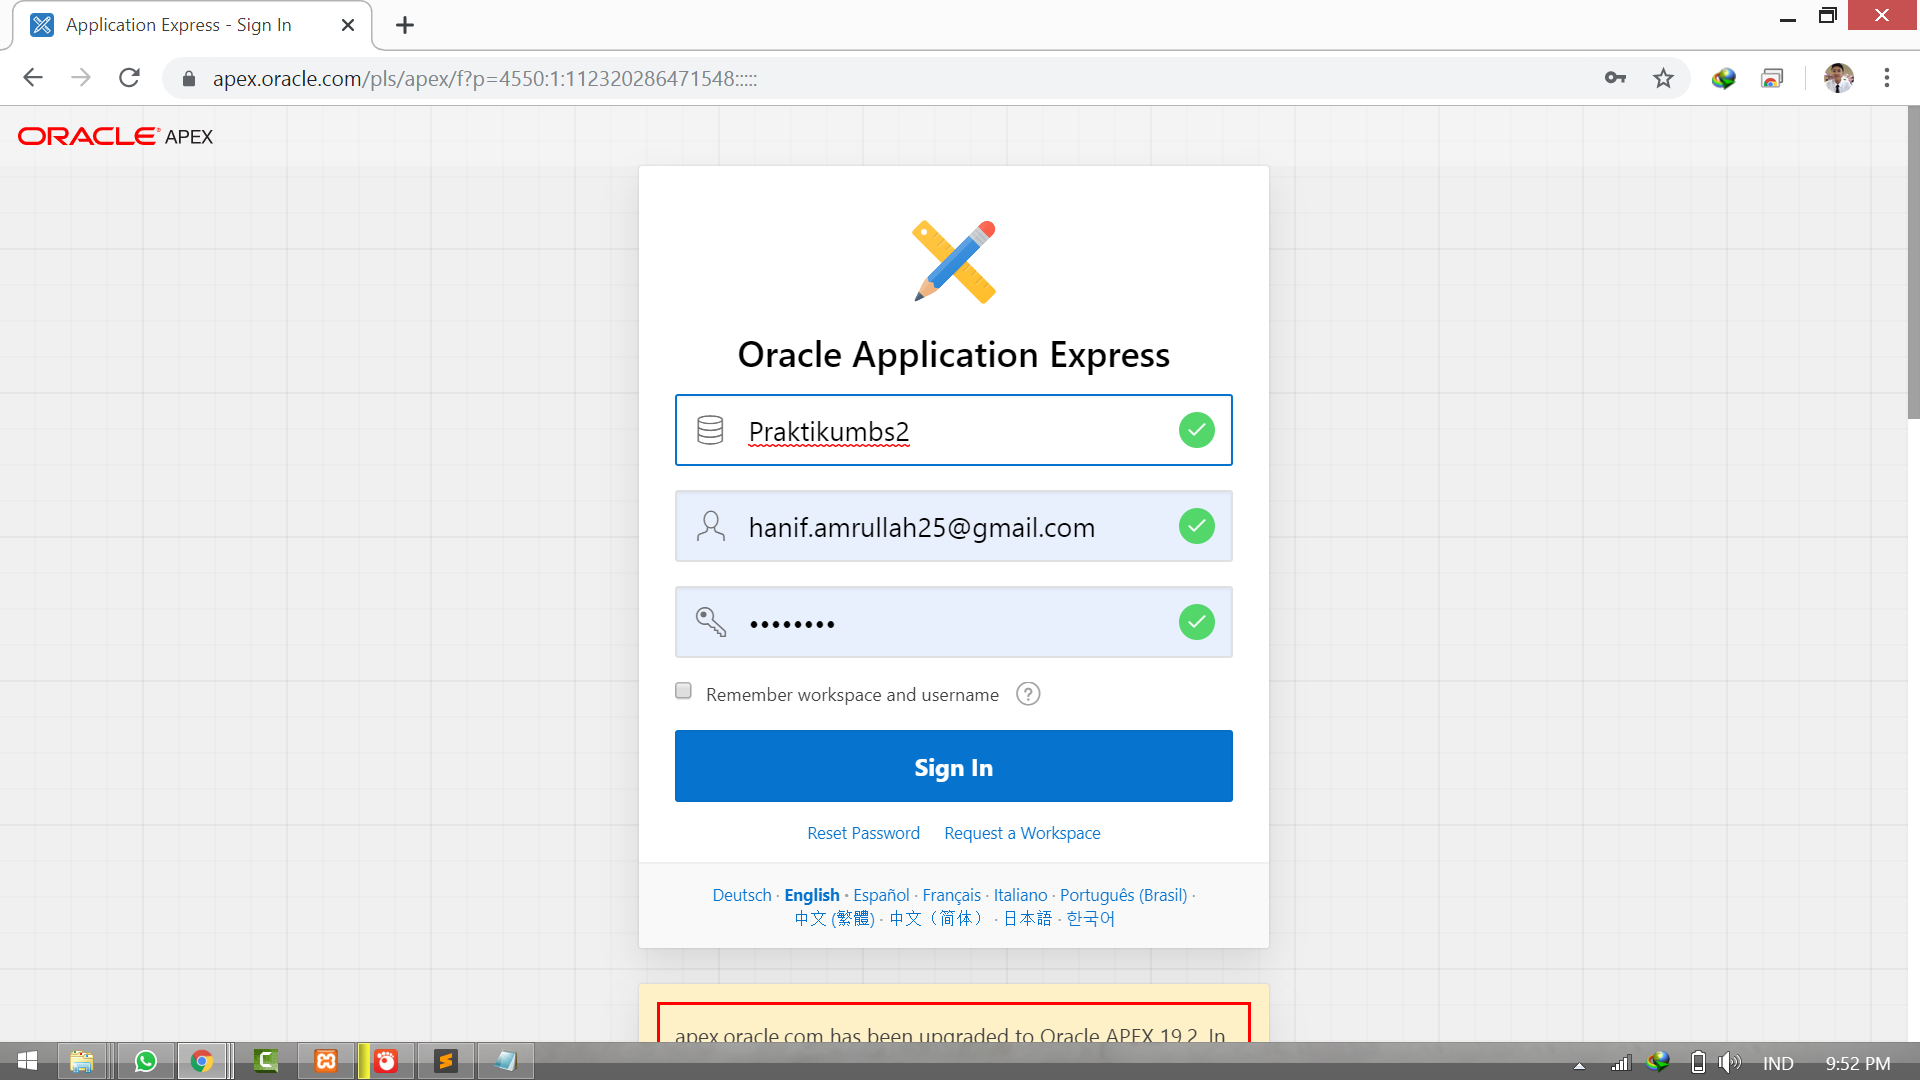
\includegraphics[width=11cm\textwidth]{1.png}
    \end{center}
    \item Klik Create a New App
\end{enumerate}
\subsection{Memilih Jenis Aplikasi}
\begin{enumerate}
    \item Klik From a File
\end{enumerate}
 \begin{center}
    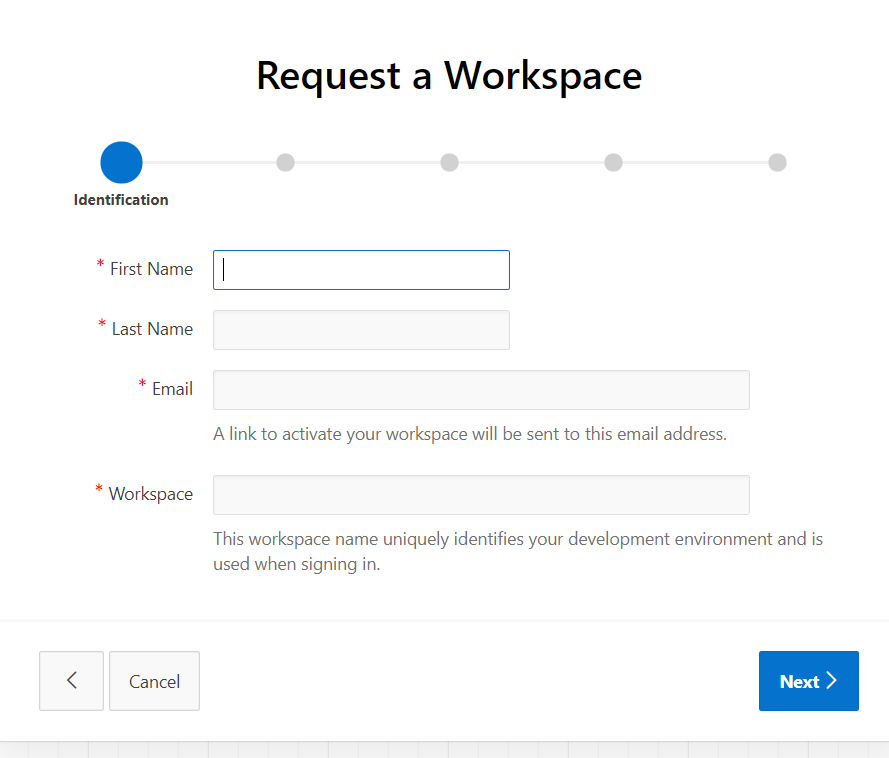
\includegraphics[width=11cm\textwidth]{3.png}
    \end{center}
\subsection{Memuat Data Sempel}
\begin{enumerate}
    \item Klik Copy and Paste 
    \item Untuk sampel data pilih Project and Task
    \item Klik Next
    \begin{center}
    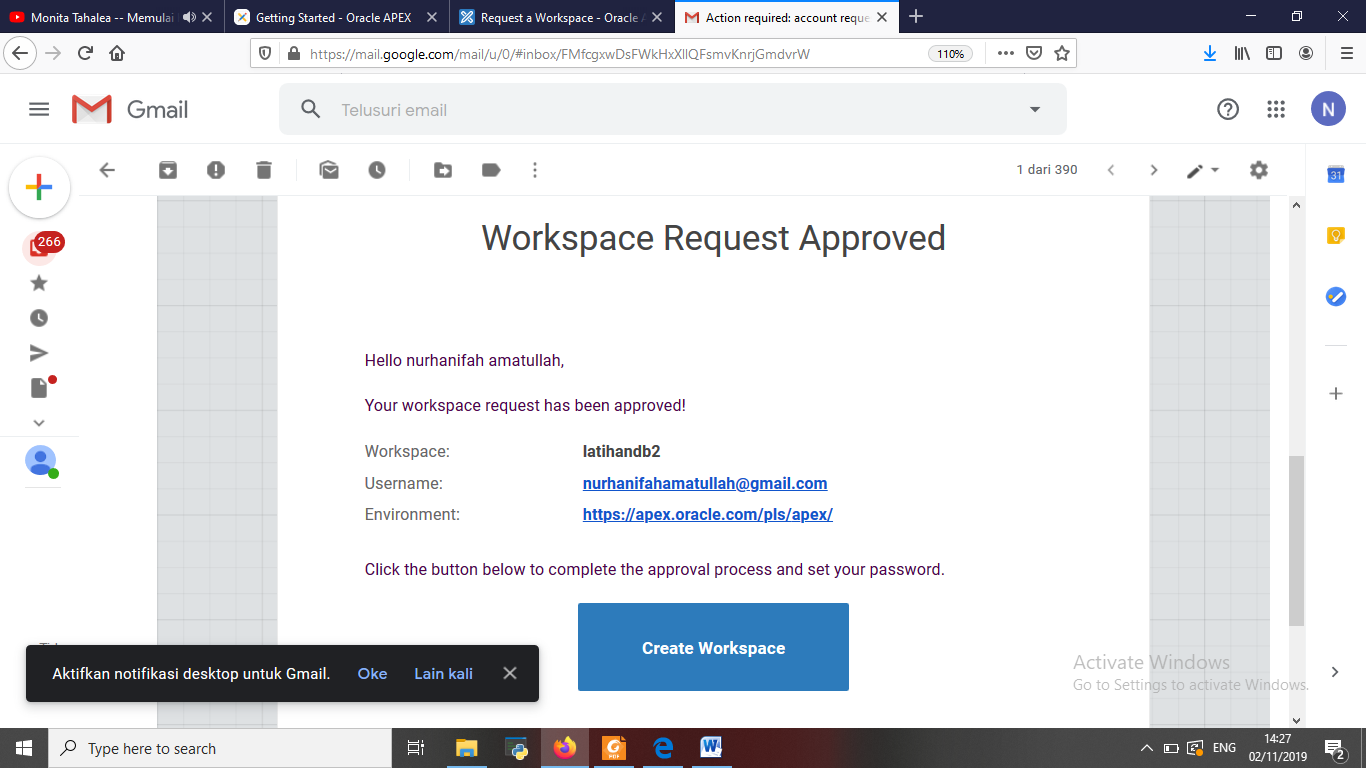
\includegraphics[width=11cm\textwidth]{6.png}
    \end{center}
\end{enumerate}
\subsection{Menamai Table}
\begin{enumerate}
    \item Pilih Table Name (Spreadsheet)
    \begin{center}
    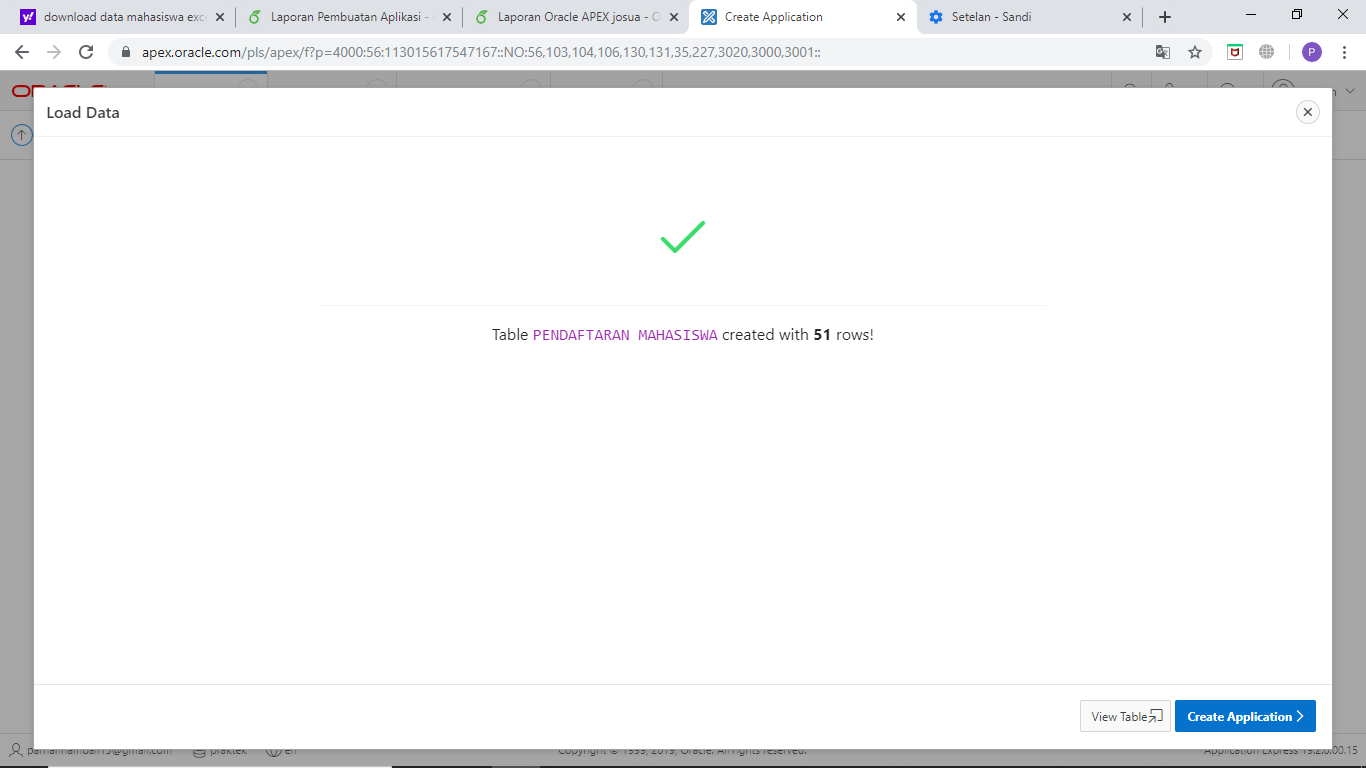
\includegraphics[width=11cm\textwidth]{8.png}
    \end{center}
    \item klik Load
\end{enumerate}
\subsection{Memverivikasi Catatan yang Dimuat}
\begin{enumerate}
    \item Periksa apakah 73 baris telah terisi
    \item klik continue to Create Application Wizard
    \begin{center}
    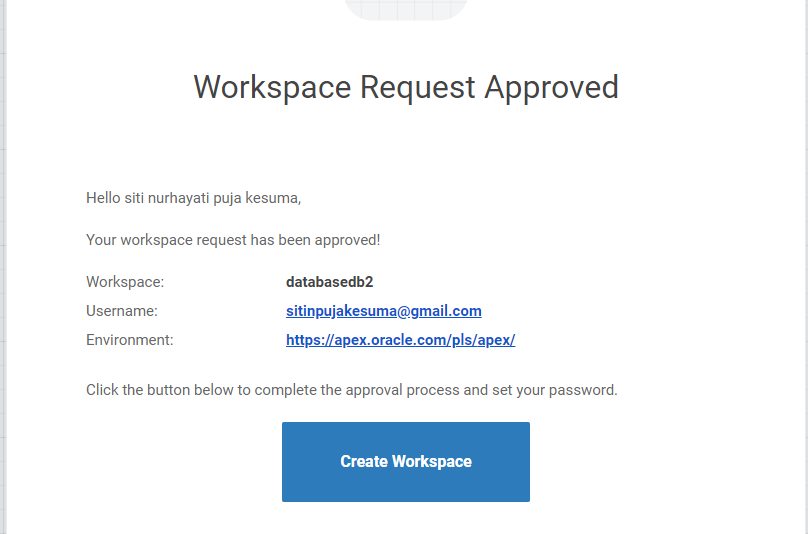
\includegraphics[width=11cm\textwidth]{10.png}
    \end{center}
\end{enumerate}
\subsubsection{Memberi Nama Aplikasi}
\begin{enumerate}
    \item pilih Name (App From A Spreadsheet)
    \begin{center}
    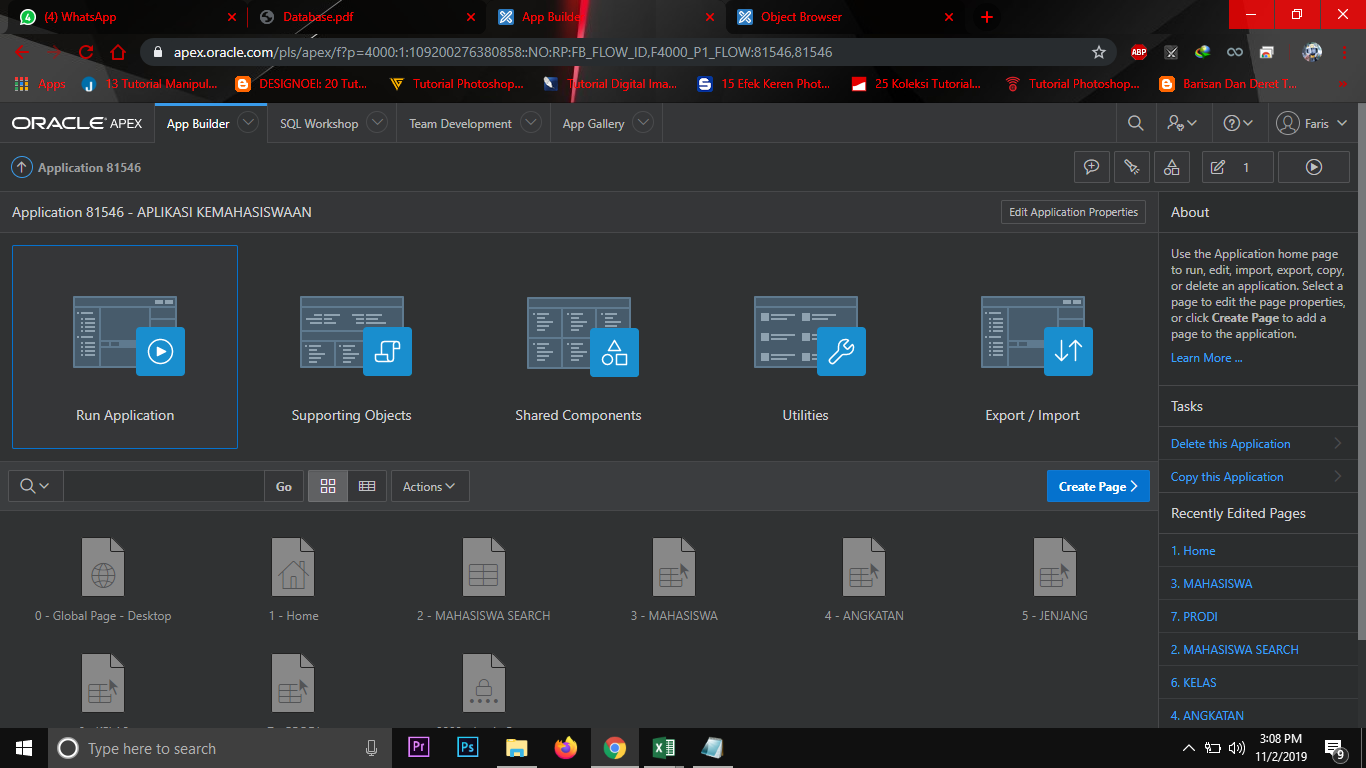
\includegraphics[width=11cm\textwidth]{11.png}
    \end{center}
    \item Lalu scrol kebawah pada Features, Klik Cheack All
    \begin{center}
    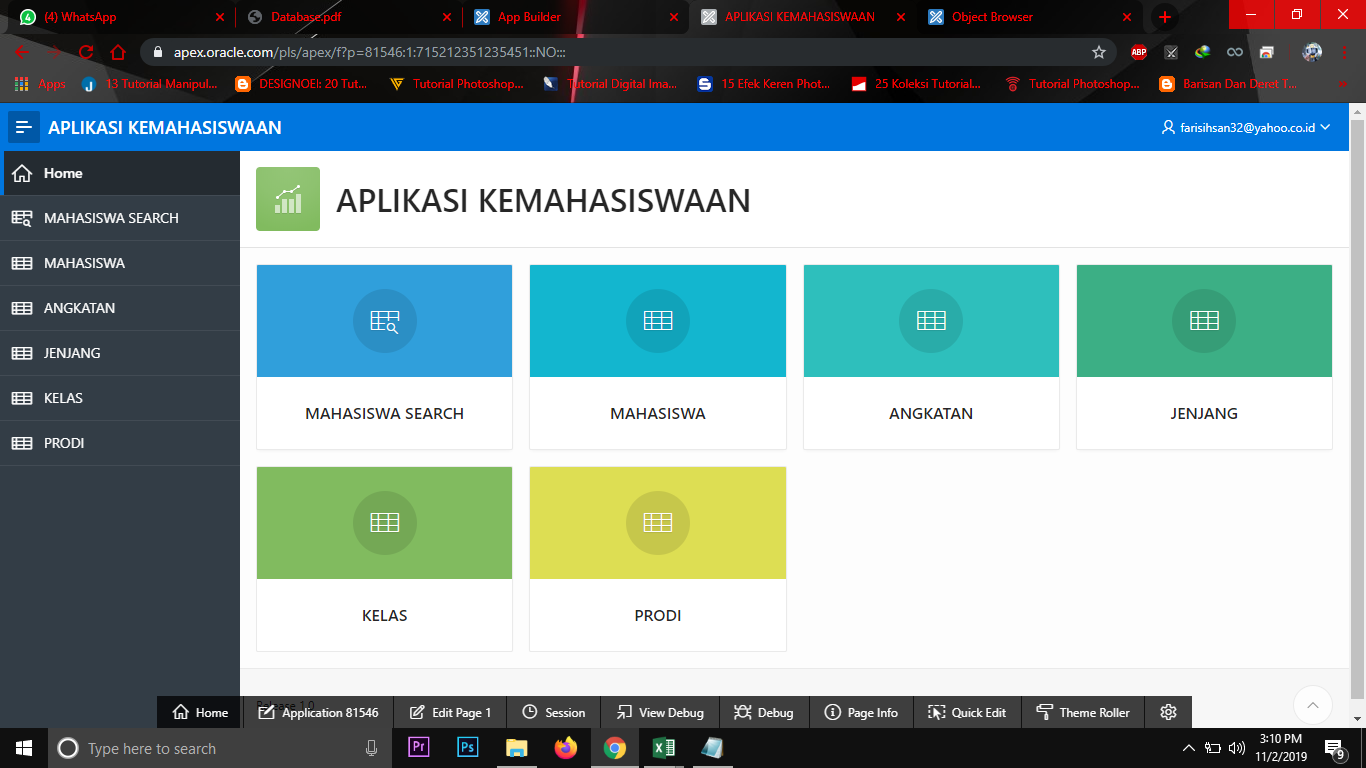
\includegraphics[width=11cm\textwidth]{12.png}
    \end{center}
\end{enumerate}
\subsection{Membuat Aplikasi}
\begin{enumerate}
    \item Pilih Create An Application
\end{enumerate}
\subsection{App In Page Desaigner}
\begin{enumerate}
    \item Aplikasi baru akan ditampilkan pada Page Desaigner
    \item Klik Run Aplikasi
    \begin{center}
    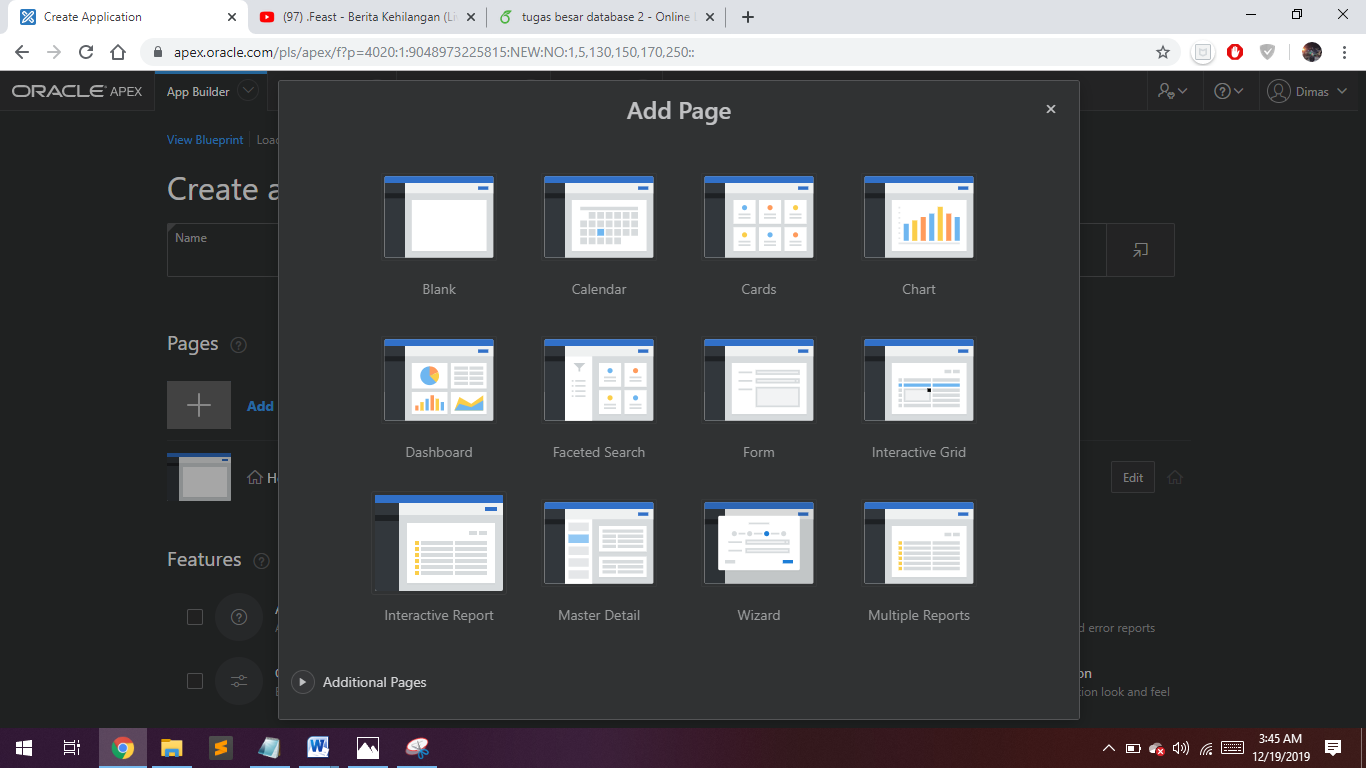
\includegraphics[width=11cm\textwidth]{14.png}
    \end{center}
\end{enumerate}
\subsection{Runtime Aplikasi}
\begin{enumerate}
    \item Masukkan User Credentials anda
    \item Cobalah Aplikasi Baru Anda
    \begin{center}
    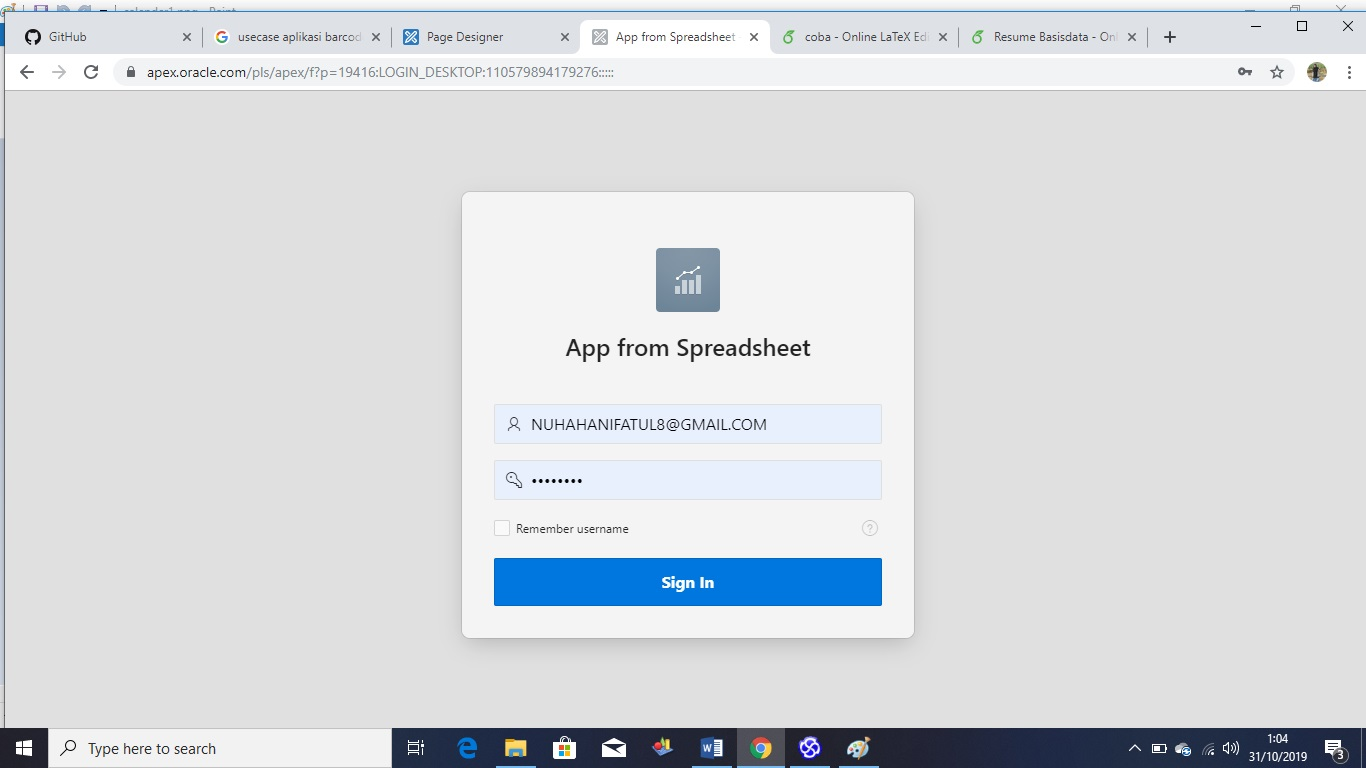
\includegraphics[width=11cm\textwidth]{user credensial.jpg}
    \end{center}
\end{enumerate}

\section{Menggunakan Runtime Environment}
\subsection{Mengurutkan Laporan Interaktif}
\begin{enumerate}
    \item Klik Spreadsheet
    \begin{center}
    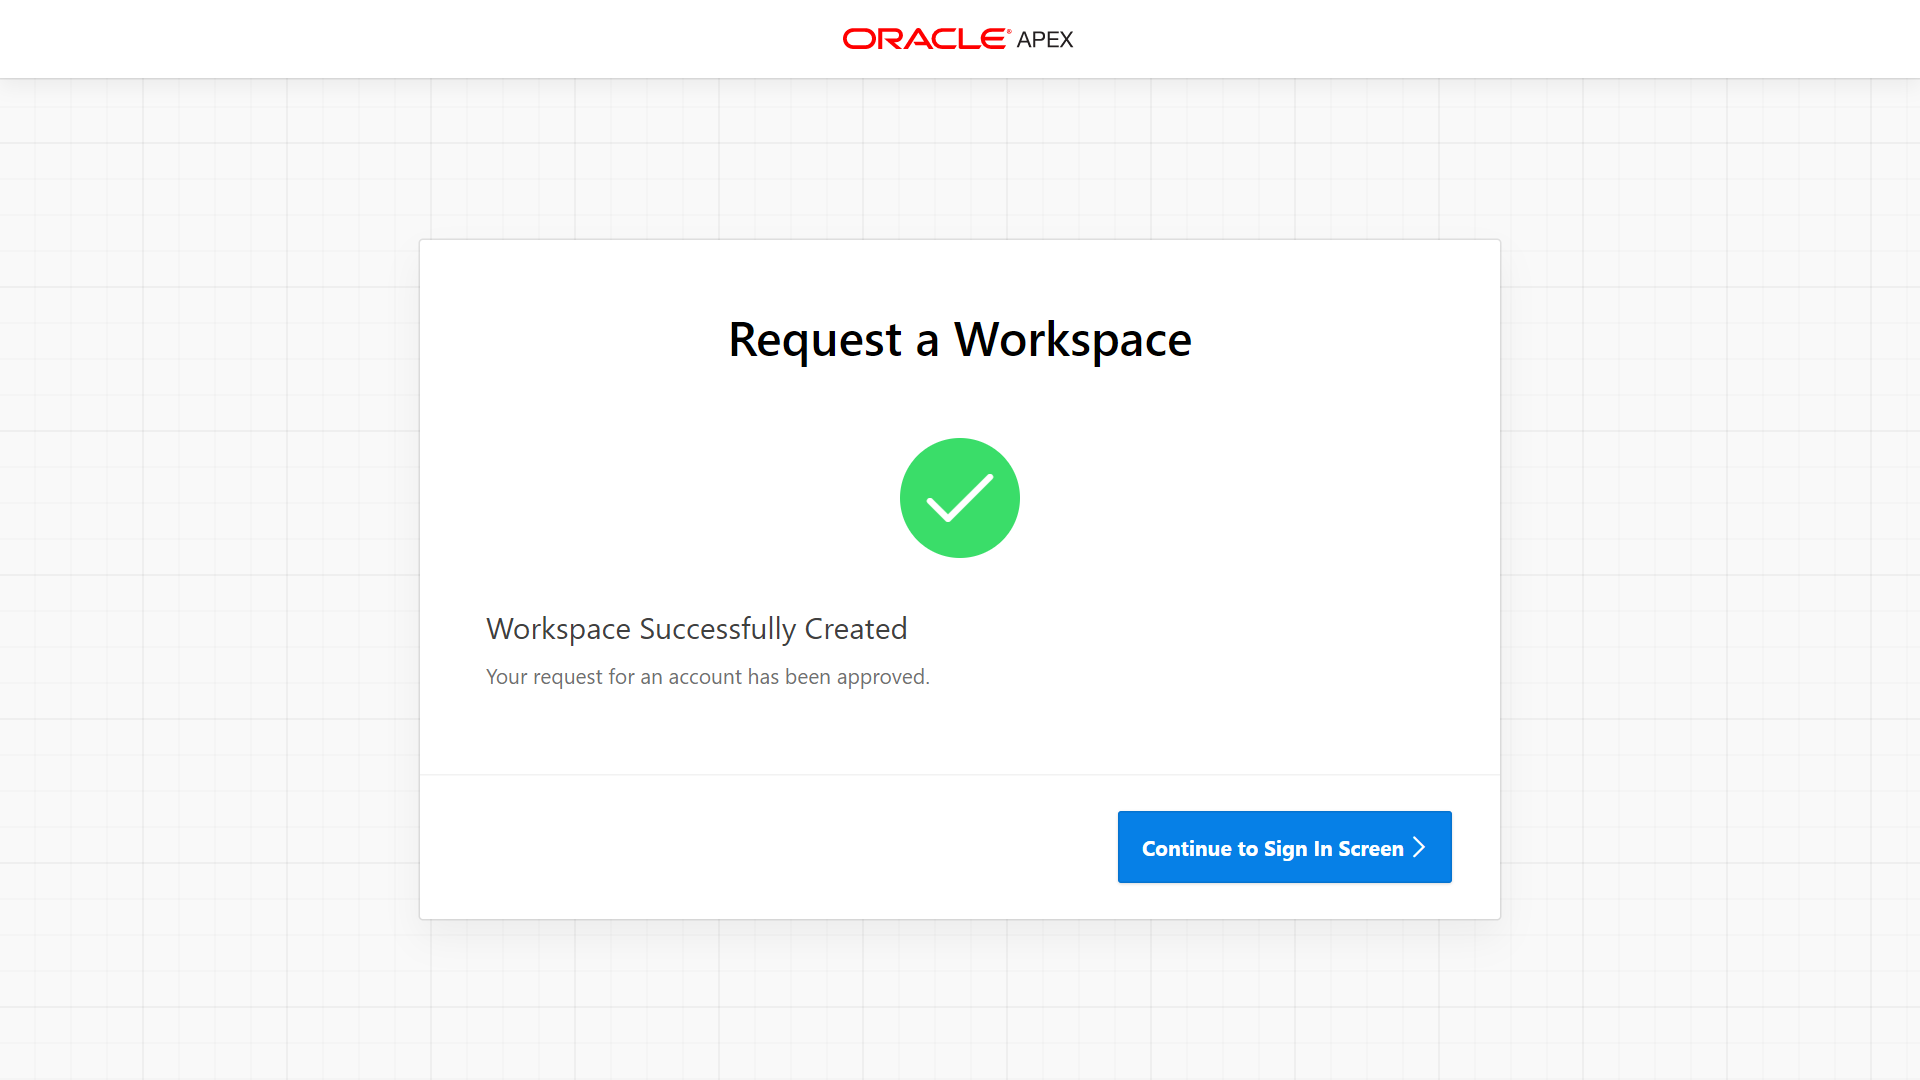
\includegraphics[width=11cm\textwidth]{15.png}
    \end{center}
    \item Clik Actions, Select Data, Select Sort
    \begin{center}
    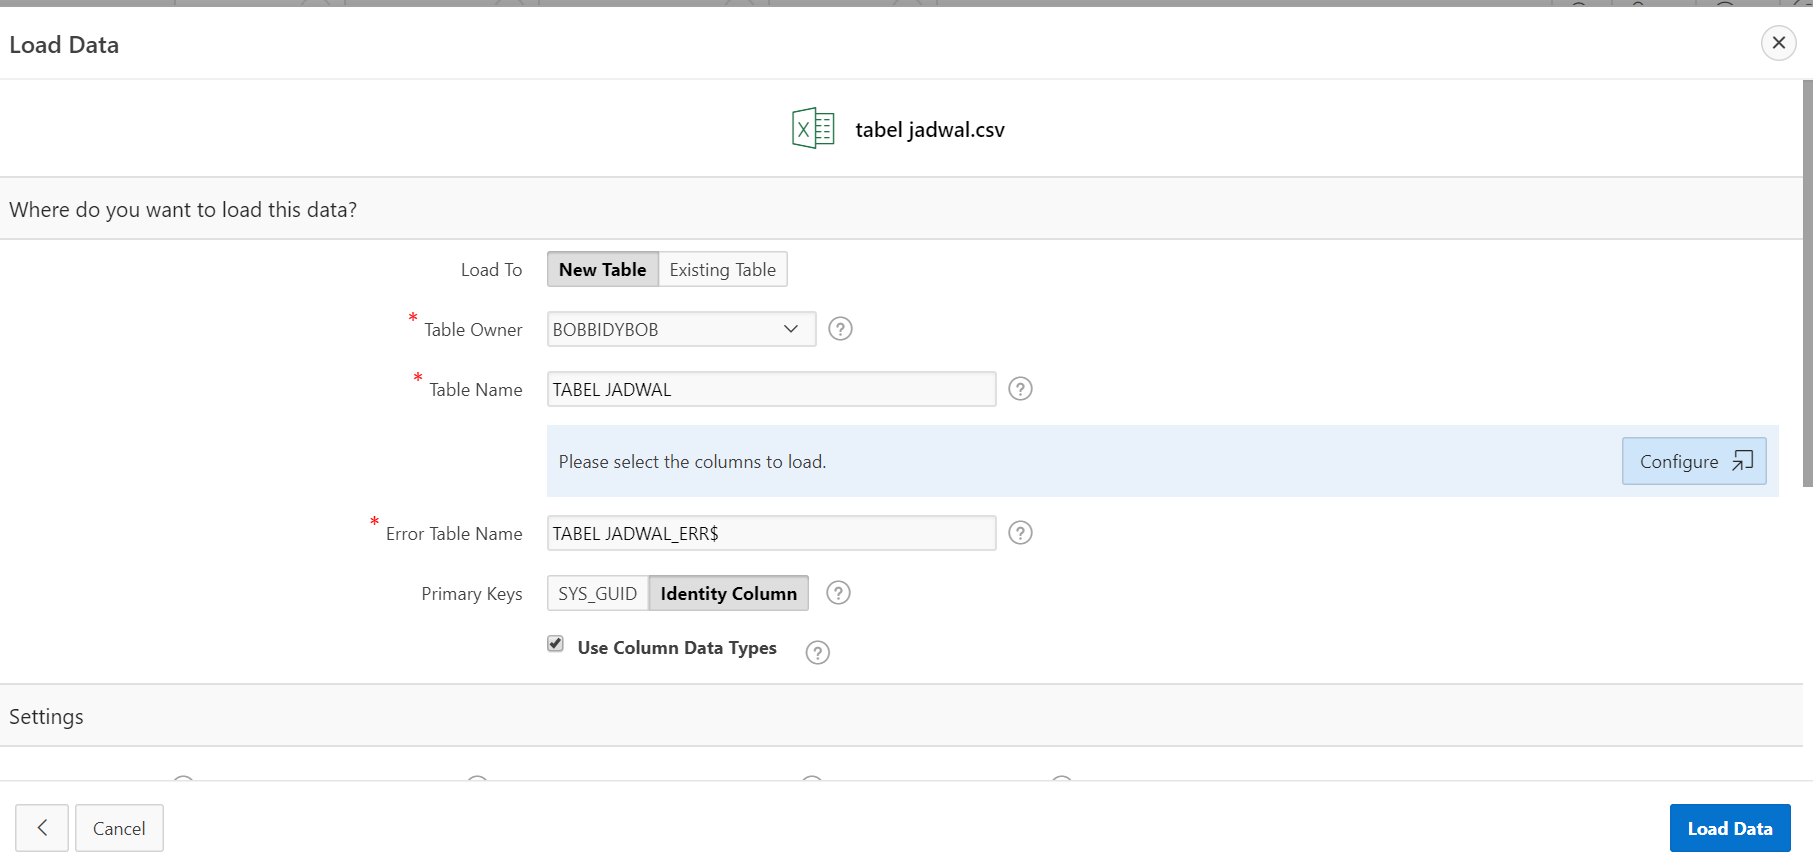
\includegraphics[width=11cm\textwidth]{16.png}
    \end{center}
    \item kolom pertama, Select Start Date; kolom kedua, Select End Date; Clik Apply
    \begin{center}
    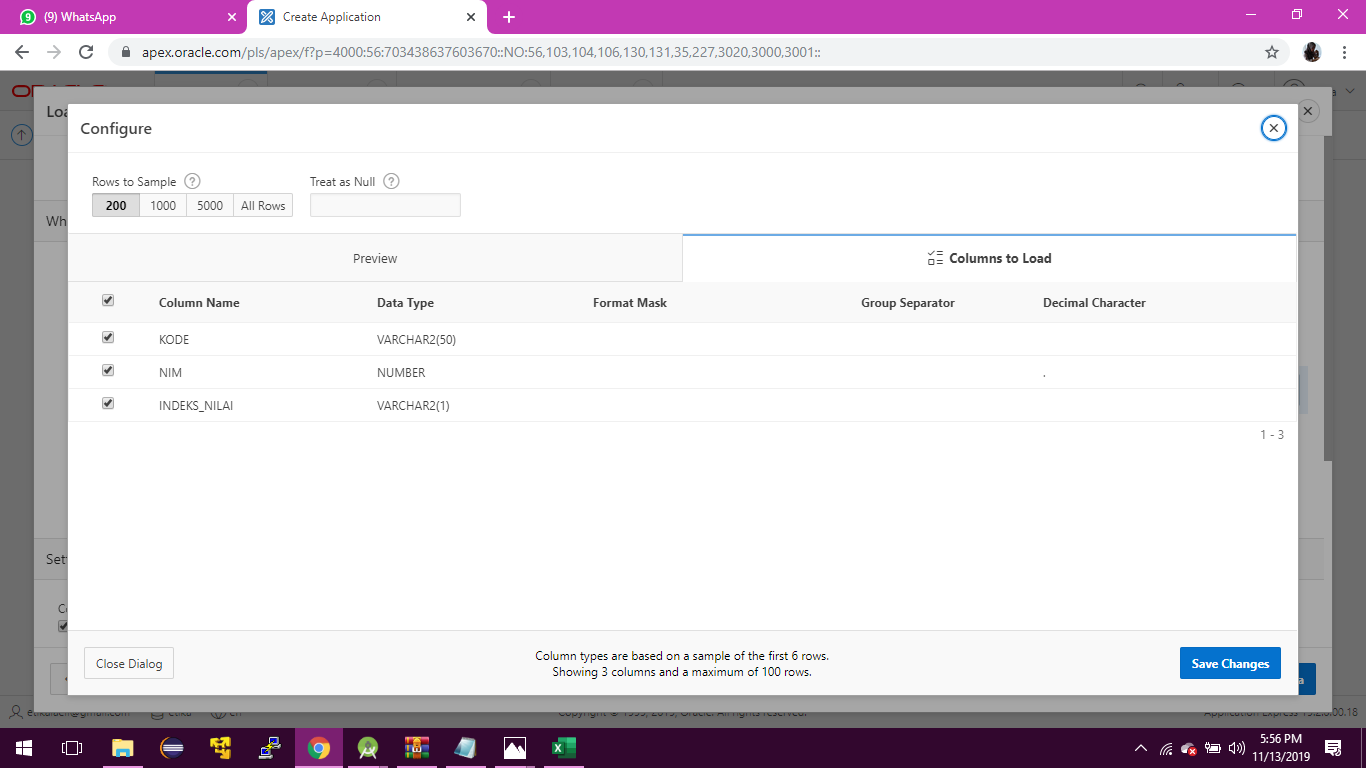
\includegraphics[width=11cm\textwidth]{17.png}
    \end{center}
\end{enumerate}
\subsection{Menambah Komputasi}
\begin{enumerate}
    \item Klik Actions, select Data, select Compute
    \begin{center}
    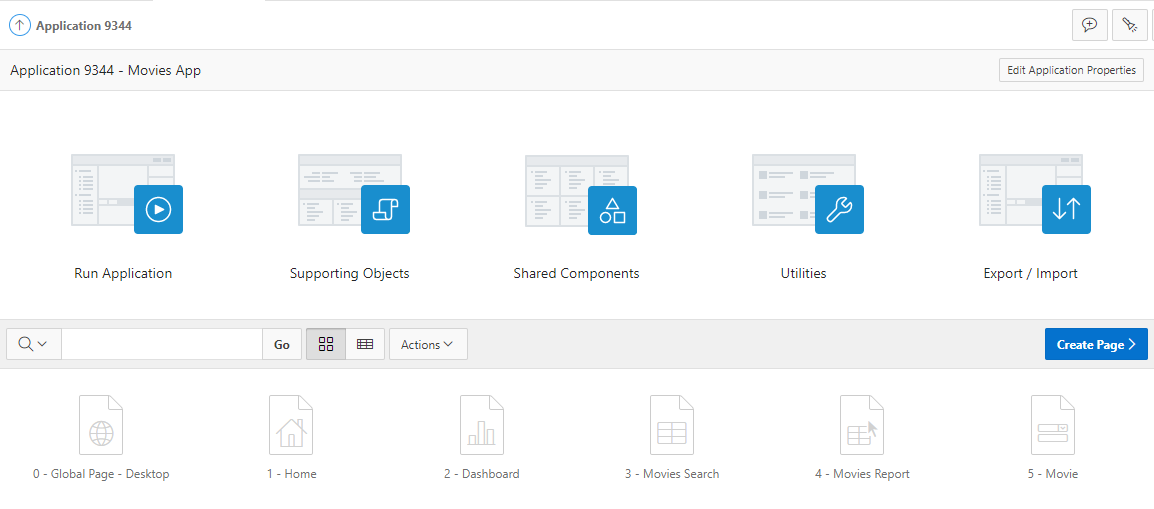
\includegraphics[width=11cm\textwidth]{18.png}
    \end{center}
    \item Column Label Masukan Budget V Cost
    \item Format Mask pilih 5,243,10
    \item Masukkan Ekspresi Komputasi I-H
    \item Klik Apply
    \begin{center}
    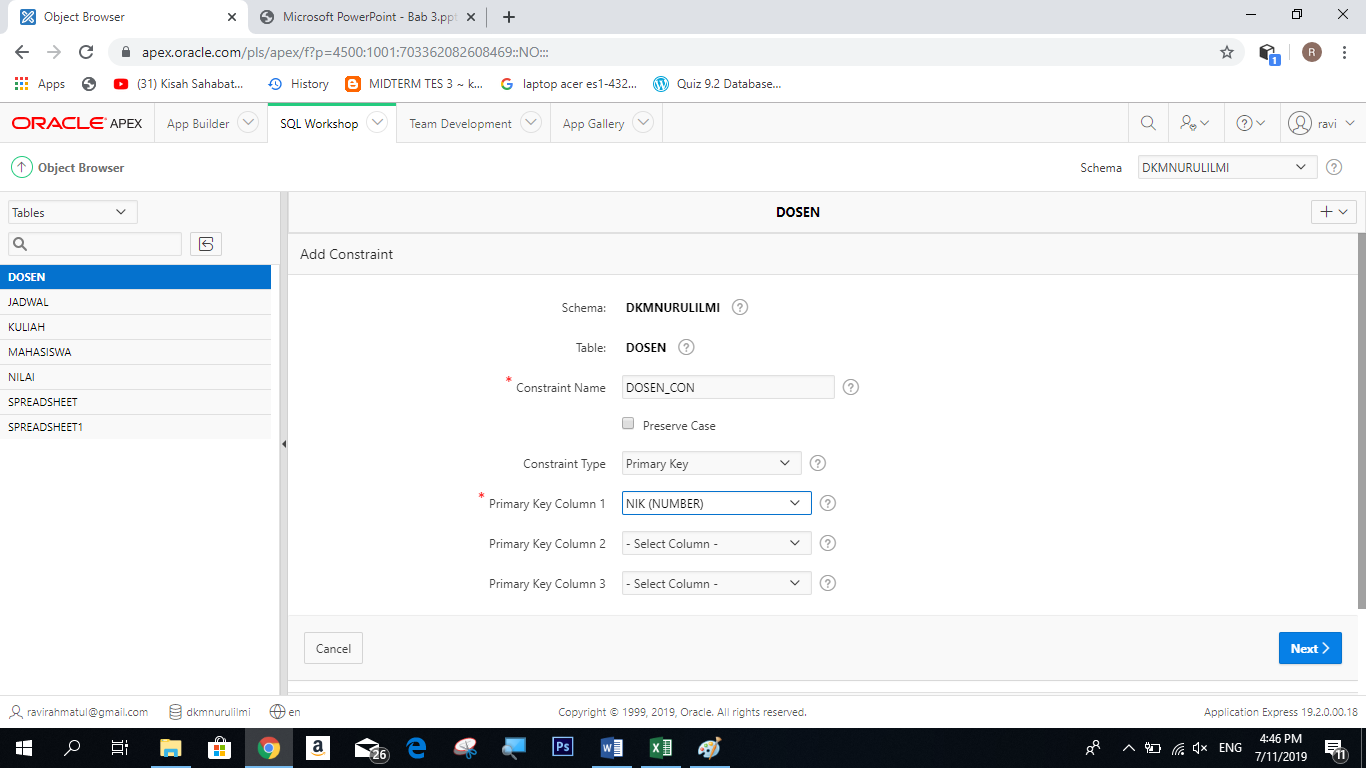
\includegraphics[width=11cm\textwidth]{19.png}
    \end{center}
\textit {NB: Untuk Pengeditan Grafik Bisa Dilakukan Didalam App From Spreadsheet}
\end{enumerate}
\subsection{Menyimpan laporan}
\begin{enumerate}
    \item Klik”Action”,Pilih “Report”, Pilih”Save Report”
    \item Untuk Simpan, Pilih “As Default Report Settings”
    \item  Tipe Default Laporan, Pilih “ Alternative”
    \item Nama, Enter “Data Review”
    \item Klik “Apply”
\end{enumerate}
\subsection{Menambahkan Sebuah Grafik}
\begin{enumerate}
    \item Klik “Action”, Dan Pilih “Chart”
    \item pada dialog Chart Pilih “**Budget V Cost”
    \item Fungsi Pilih “ Sum”
    \item Sort Pilih “Label-Ascending”
    \item Orientasi Pilih “Horizontal”
    \item Klik “Apply”
     \begin{center}
    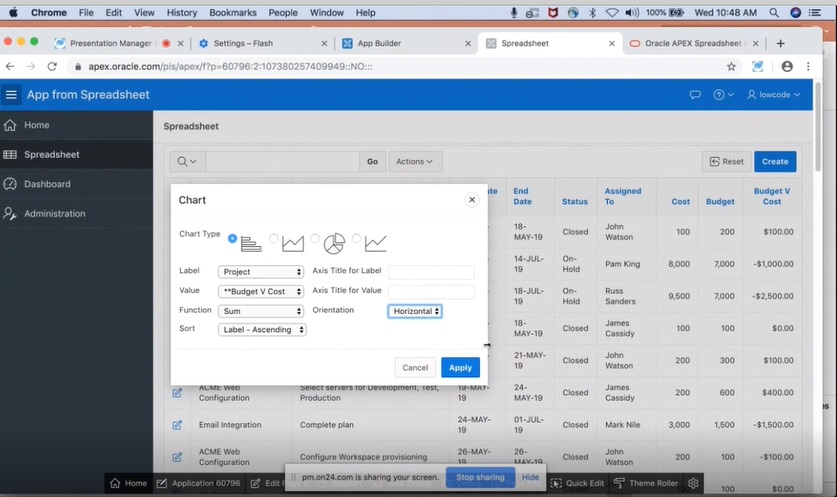
\includegraphics[width=11cm\textwidth]{add grafik.jpg}
    \end{center}
\textbf{*NB: Untuk Pengeditan Grafik Bias Dilakukan Dilaman App From Spreadsheet}
\end{enumerate}
\subsection{Menyimpan Laporan}
\begin{enumerate}
    \item Klik”Action”,Pilih “Report”, Pilih”Save Report”
    \item Untuk Simpan, Pilih “As Default Report Settings”
    \item Tipe Default Laporan, Pilih “ Alternative”
    \item Nama, Enter “Data Review”
    \item Klik “Apply”
\end{enumerate}

\subsection{Batasi Status}
\begin{enumerate}
    \item Ketika Runtime Environment, Klik “Edit Icon On A Record”
    \item Halaman Modal Akan Tampil
    \item Pada Developer Toolbar, Klik “Quick Edit”
    \item Pada Status Item (Tunggu Sampai Outline Biru Muncul” Lalu Klik Mouse
     \begin{center}
    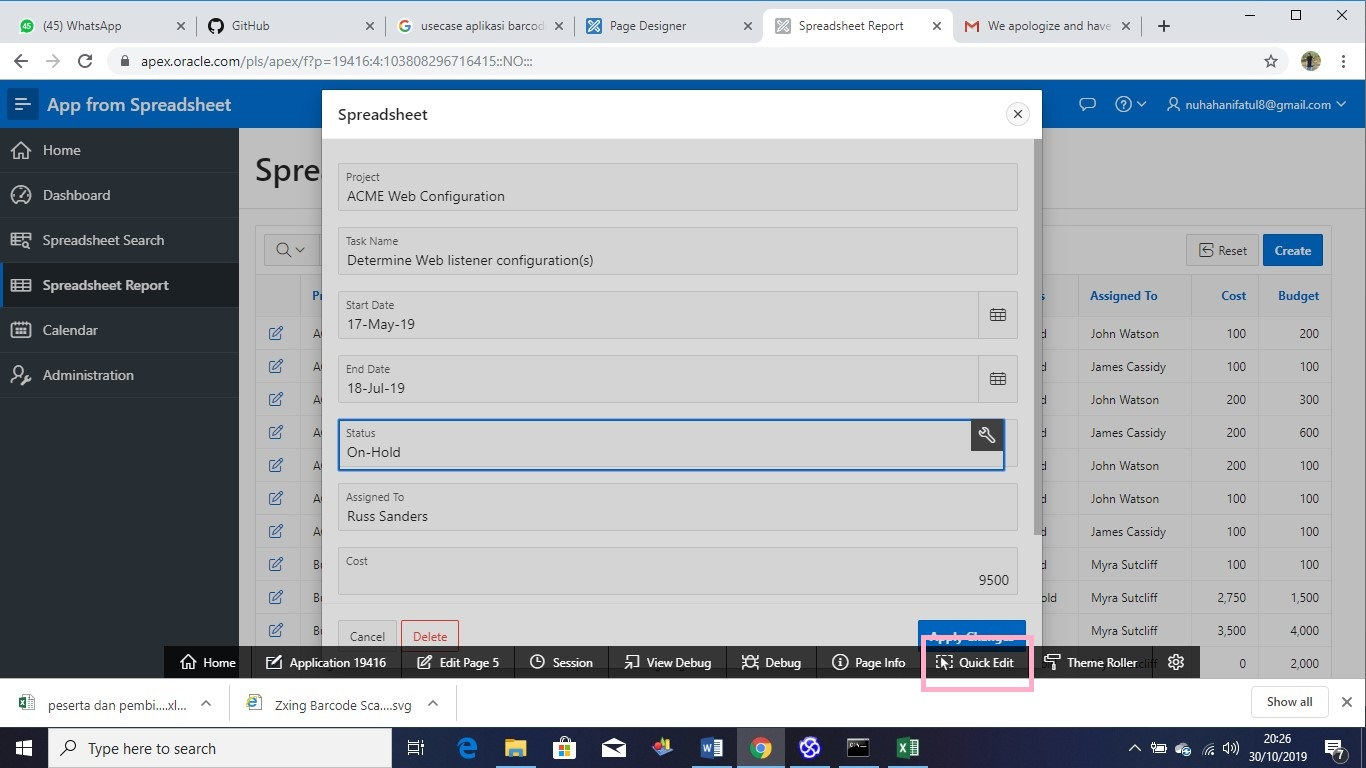
\includegraphics[width=11cm\textwidth]{membatasi status2.jpg}
    \end{center}
    \item Pada Page Designer Muncul Dengan Focus Pada Status Item
    \item Pada Page Designer, Dalam Editor Property(Panel Kanan) lalu Pada identification " Type " pilih -select list-
     \begin{center}
    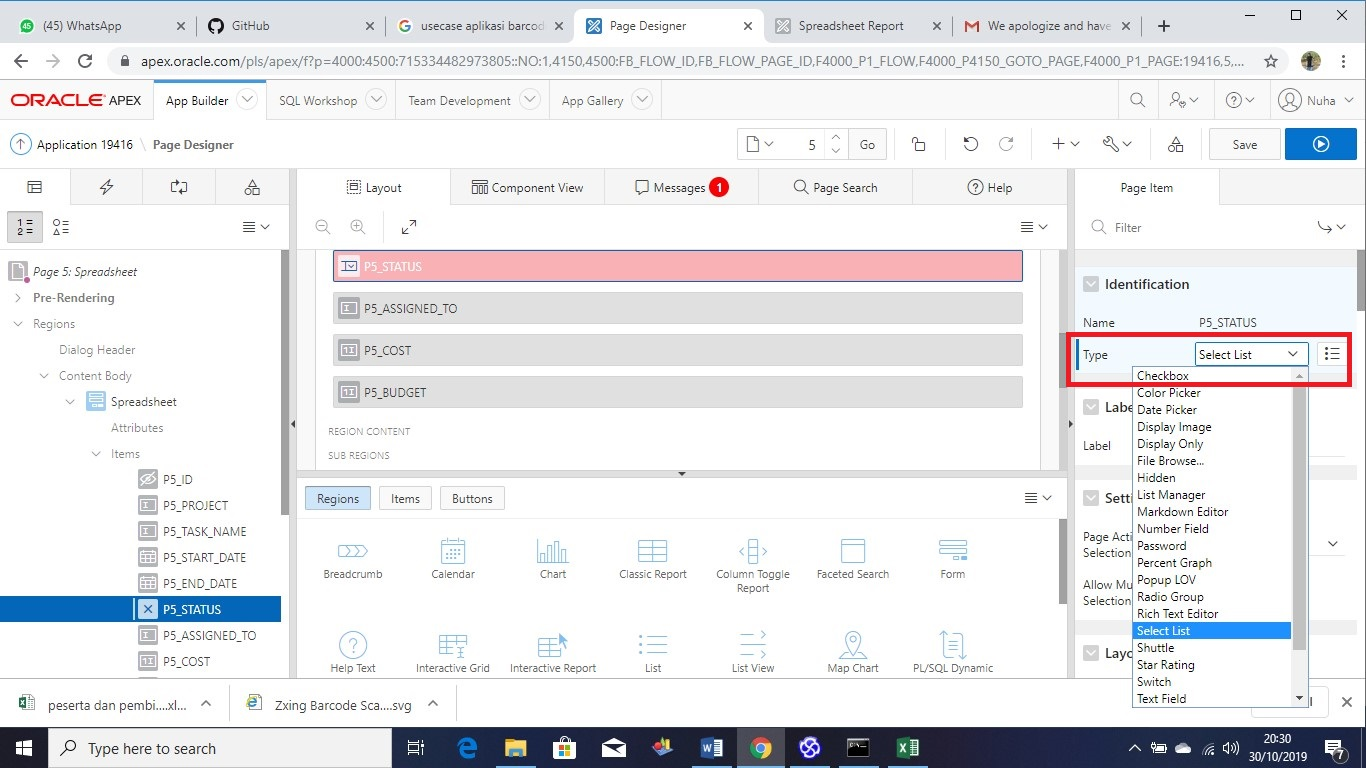
\includegraphics[width=11cm\textwidth]{identification.jpg}
    \end{center}
    \item Scroll ke bawah, Untuk "List and Values" Pilih “SQL Query”
     \begin{center}
    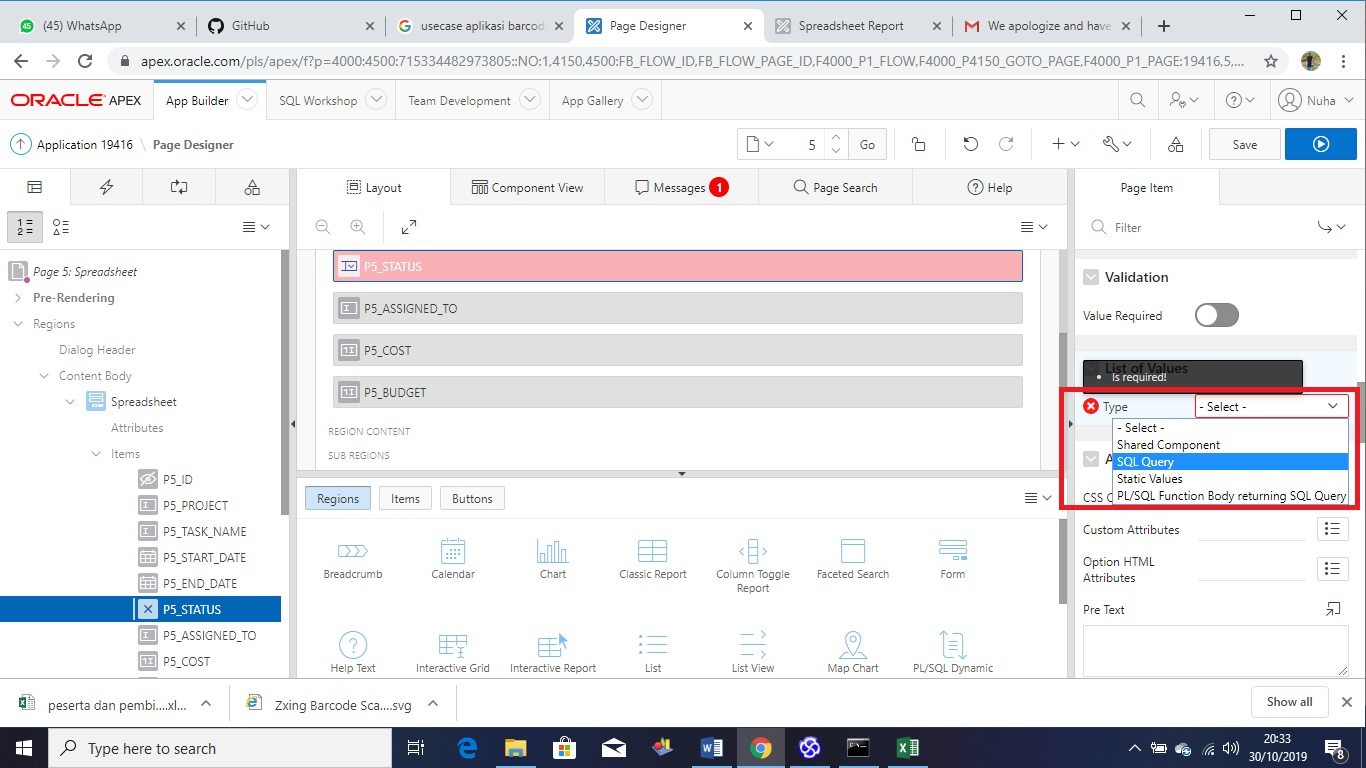
\includegraphics[width=11cm\textwidth]{sql queery.jpg}
    \end{center}
    \item Lanjutkan Ke SQL Query, Klik “Code Editor” pada kanan sebelah SQL Query
    \item Dalam Kode Masukkan Seperti Ini"
    \textit{"select distinct status d, status r from spreadsheet order by 1"}
    \item Klik Validate
    \item Klik Ok
     \begin{center}
    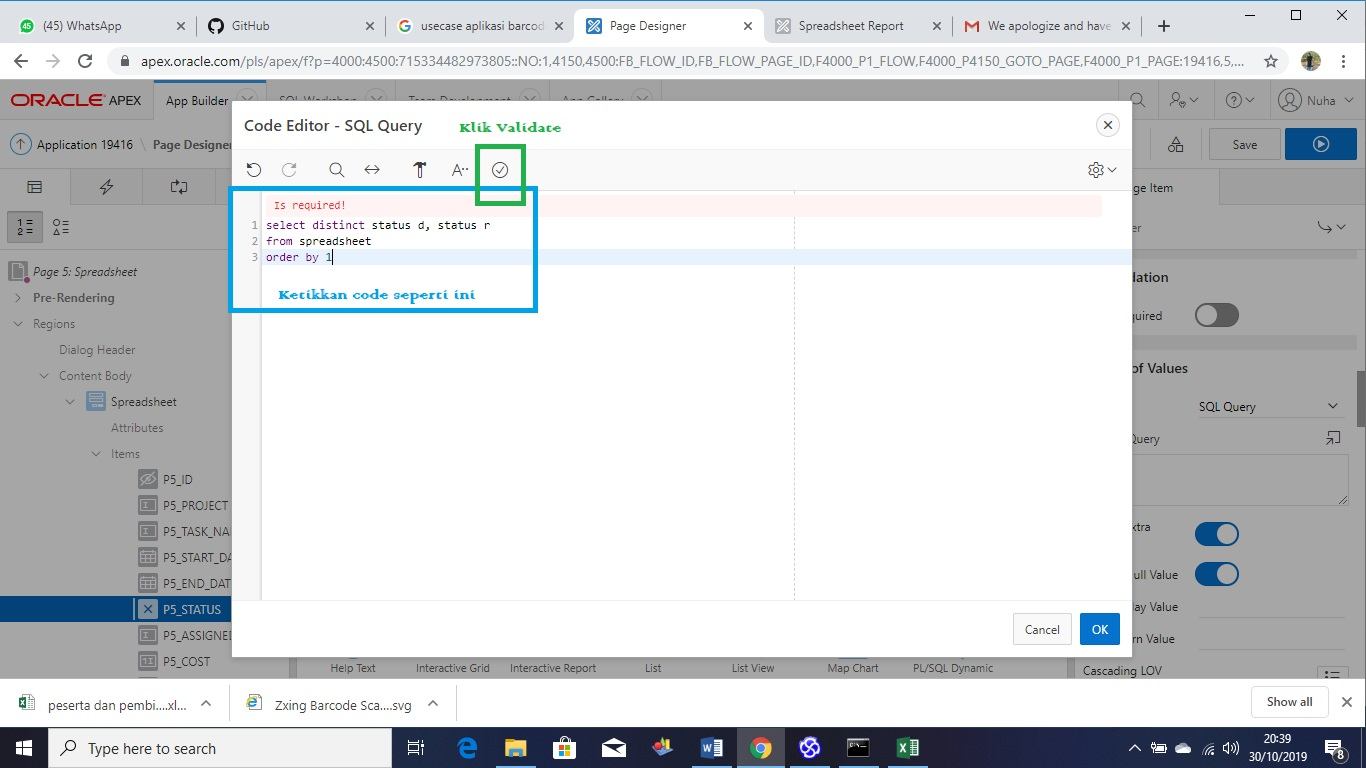
\includegraphics[width=11cm\textwidth]{codesql.jpg}
    \end{center}
    \item Pada "Vules Exstra" pilih no, pada "Null Display Value" pilih yes, dan pada "Null Display Value“ pilih -select status-.
      \begin{center}
    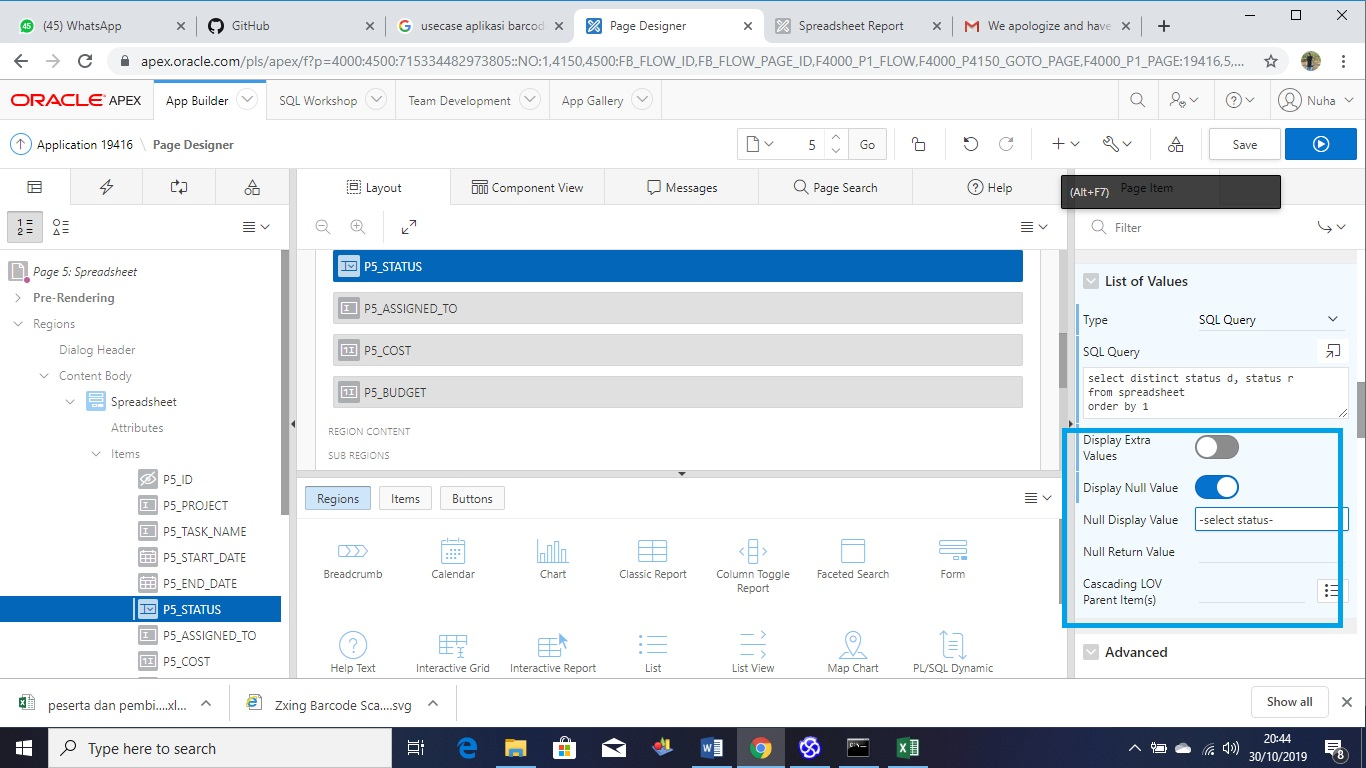
\includegraphics[width=11cm\textwidth]{value extra.jpg}
    \end{center}
    \item Klik Save (Pada Toolbar kanan atas)
\end{enumerate}
\subsection{Menjalankan Aplikasi}
\begin{enumerate}
    \item Arahkan Navigasi Ke Runtime Environment
    \item Refresh Browser
    \item Edit Record
    \item Klik Status pilih "Close"
     \begin{center}
    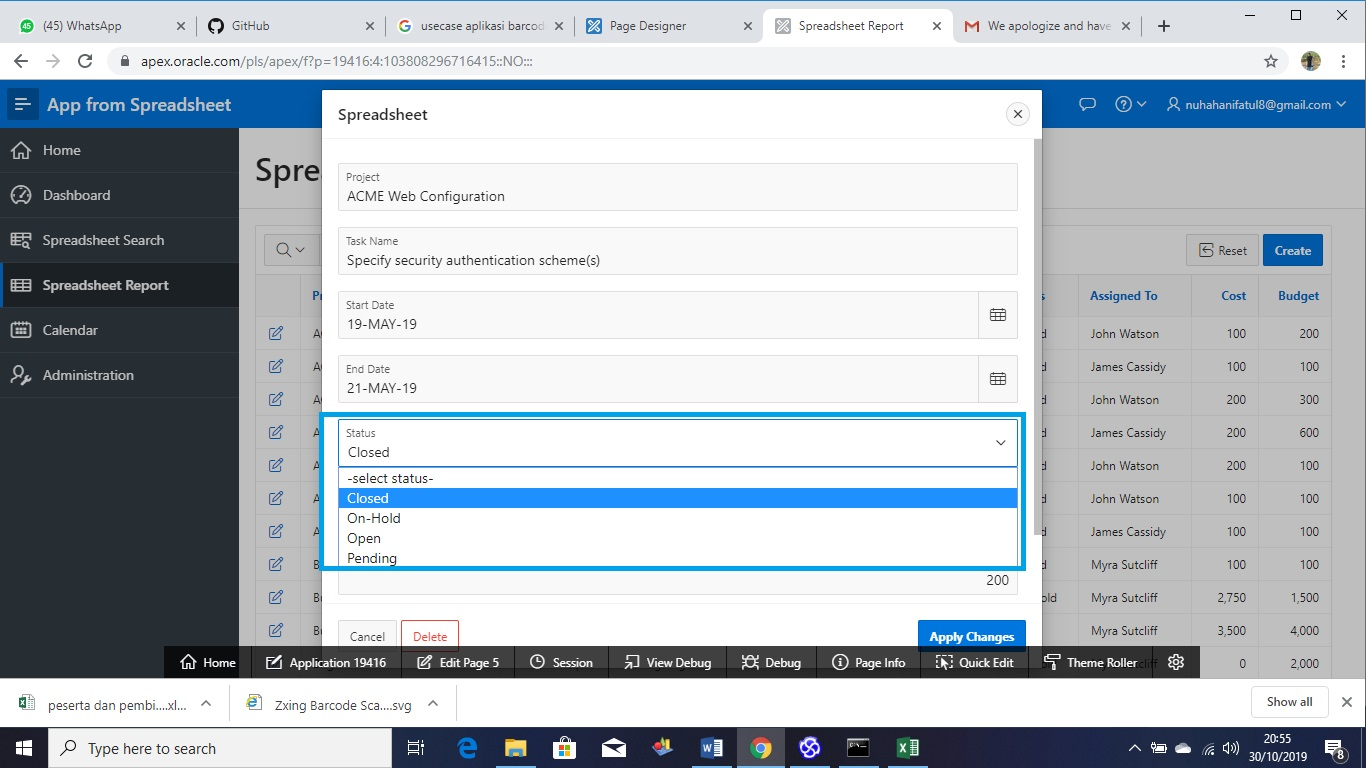
\includegraphics[width=11cm\textwidth]{Menjalankan app.jpg}
    \end{center}
\end{enumerate}

\section{Membuat Kalender}
\subsection{Menambahkan Kalender}
\begin{enumerate}
    \item Arahkan Navigasi Kembali Ke Runtime Environtment
    \item Refresh browser
    \item Pada Home pilih "Calender"
    \item Edit a Record
    \item Clik Status
    \item Pada Aplikasi Builder, Arahkan Pada Home Page
    \begin{center}
    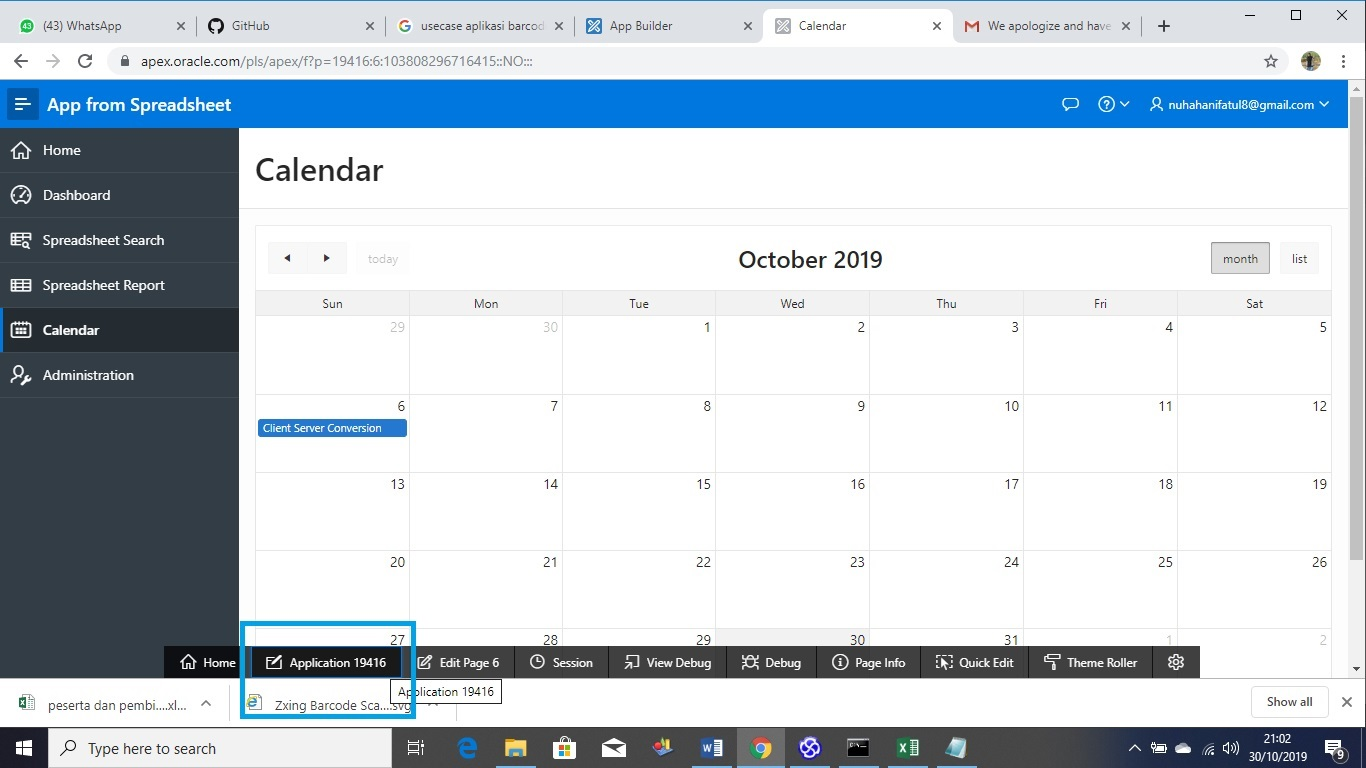
\includegraphics[width=11cm\textwidth]{app19.jpg}
    \end{center}
    \item Klik Create Page
     \begin{center}
    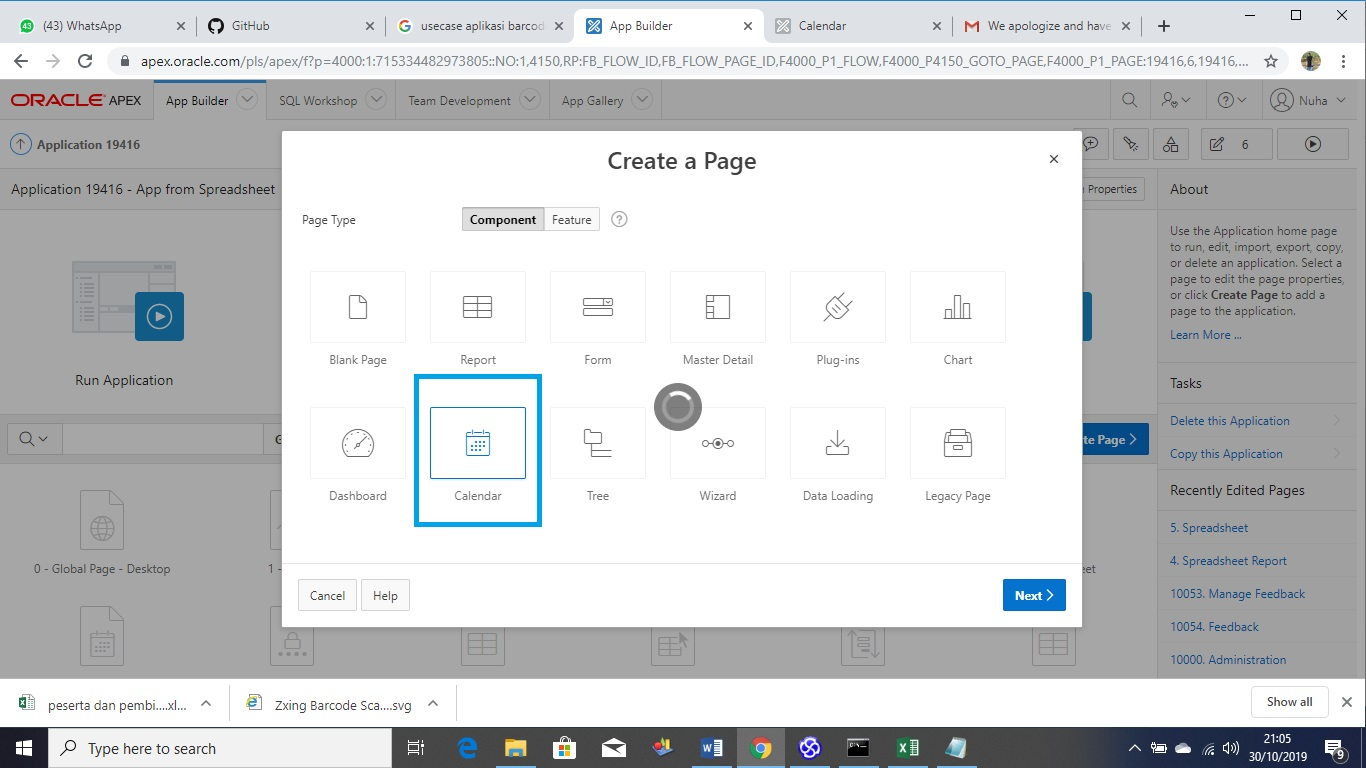
\includegraphics[width=11cm\textwidth]{create page.jpg}
    \end{center}
    \item Pilh nama  Calender
     \begin{center}
    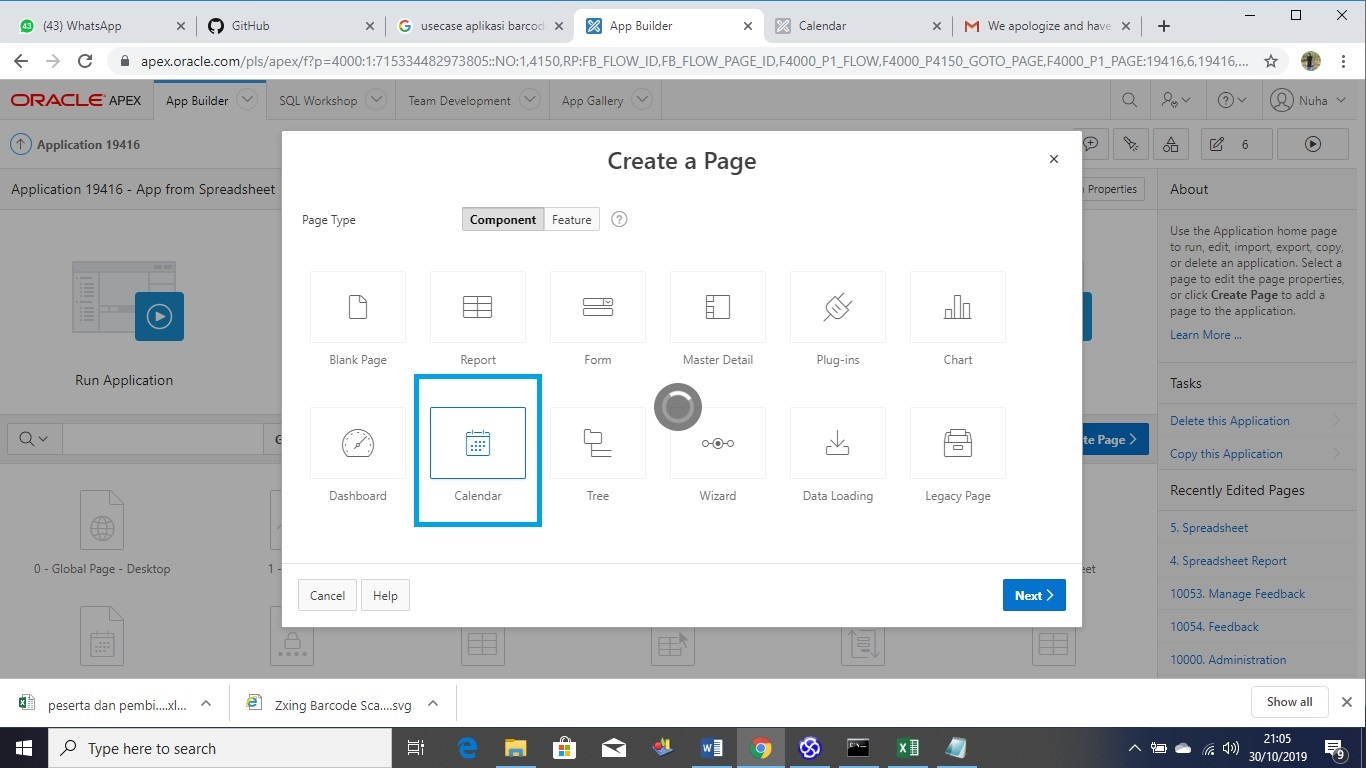
\includegraphics[width=11cm\textwidth]{calender.jpg}
    \end{center}
    \item Pada Page name “Calender”, Breadcrumb “Breadcrumb”
    \item Lalu Klik Next
     \begin{center}
    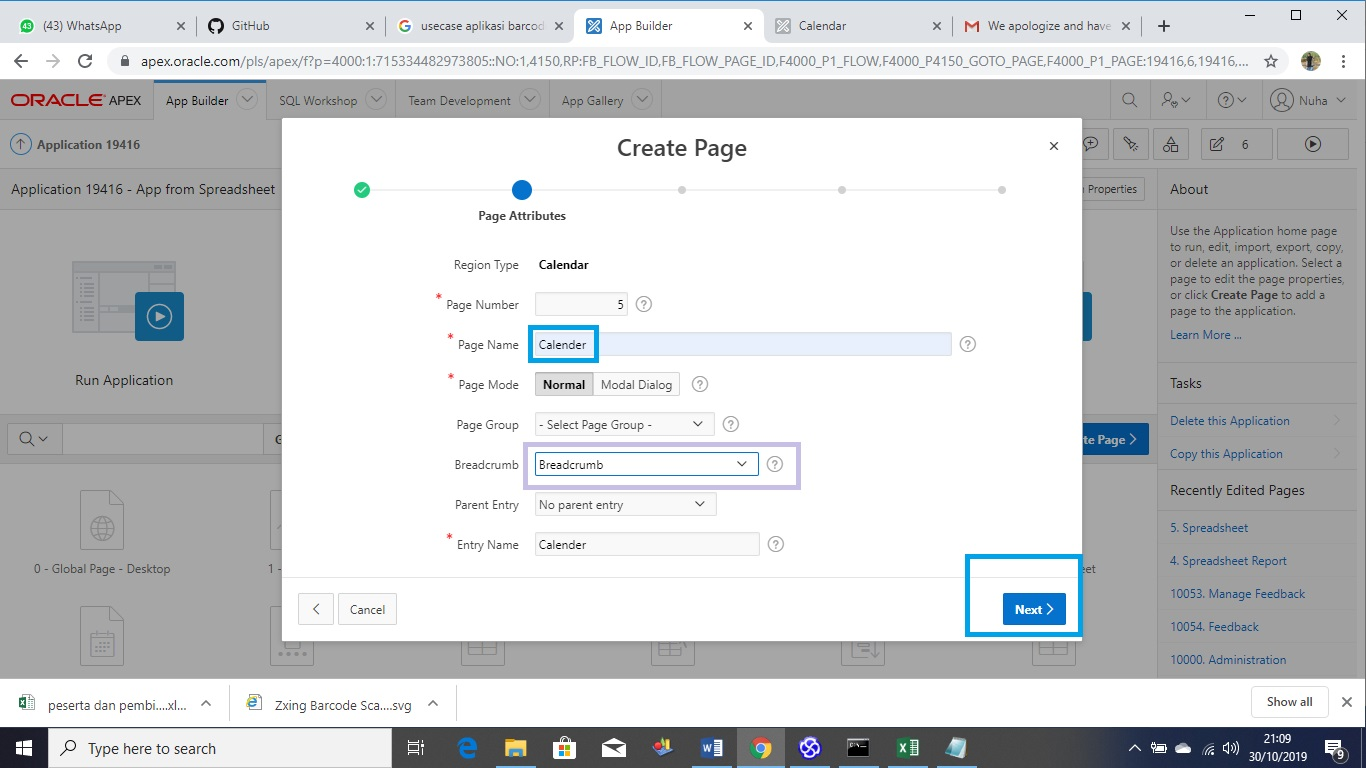
\includegraphics[width=11cm\textwidth]{calender2.jpg}
    \end{center}
    \item Pada navigasi preference klik Create a New Navigation menu Entry
    \item Selanjuknya klik Next
     \begin{center}
    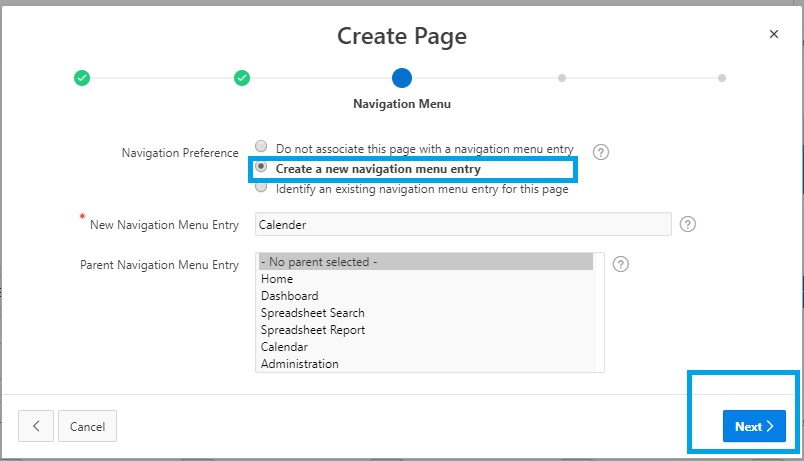
\includegraphics[width=11cm\textwidth]{calender3.jpg}
    \end{center}
    \item Pada Table / View Name pilih SPREADSHEET (table)
    \item Klik next lagi 
    \item Kolom Tampilan, Pilih TASK NAME
    \item Kolom Tanggal Akhir, Pilih END DATE	
    \item Klik Create
      \begin{center}
    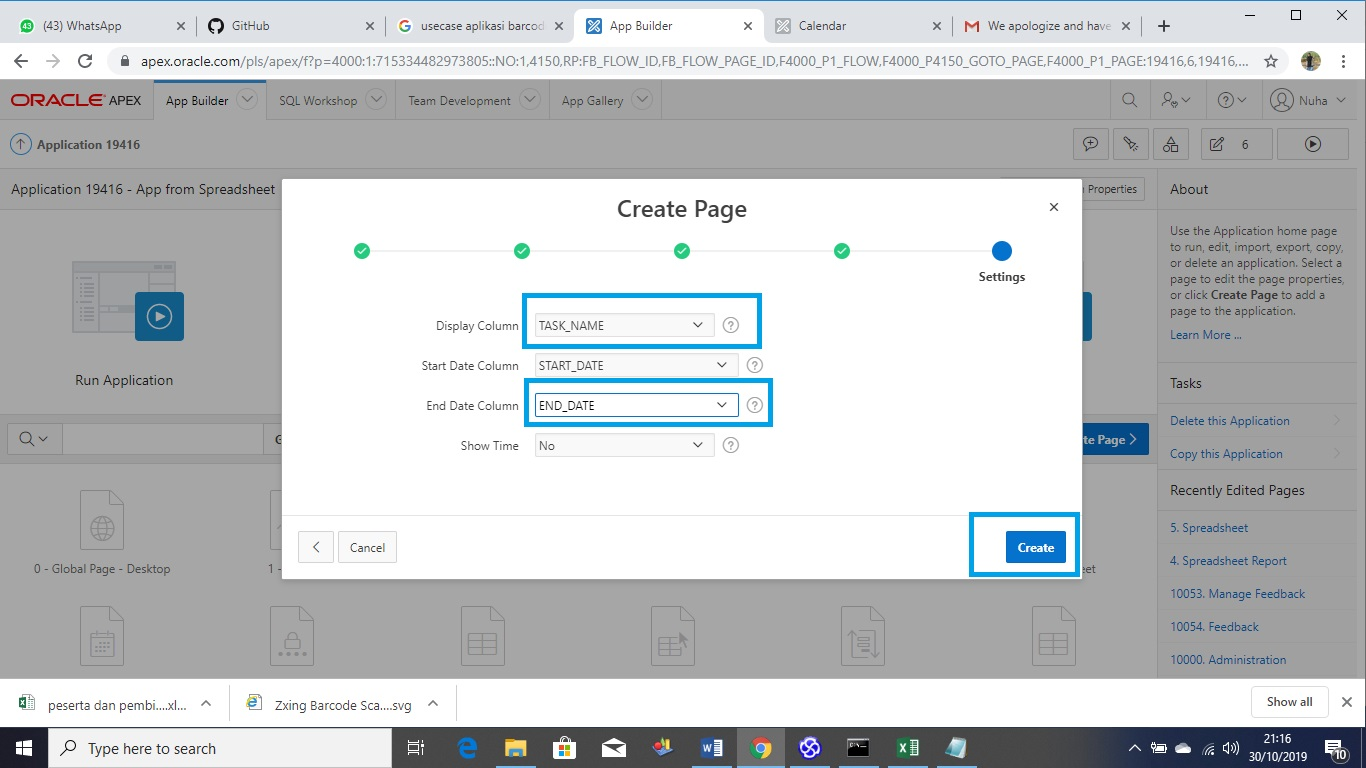
\includegraphics[width=11cm\textwidth]{calender4.jpg}
    \end{center}
\end{enumerate}
\subsection{Menautkan Kalender pada Update Form}
\begin{enumerate}
    \item Di Tab Rendering, Di Bawah Kalender, Klik Atributes
    \item Di Editor Properti (Panel Kanan), Klik View/ Edit Link
    \item Set Page "3", Items Name, Pilih "P3ID"; Nilai, Pilih ID
    \item Clear Cache, Masukkan 3
    \item Klik Ok
      \begin{center}
    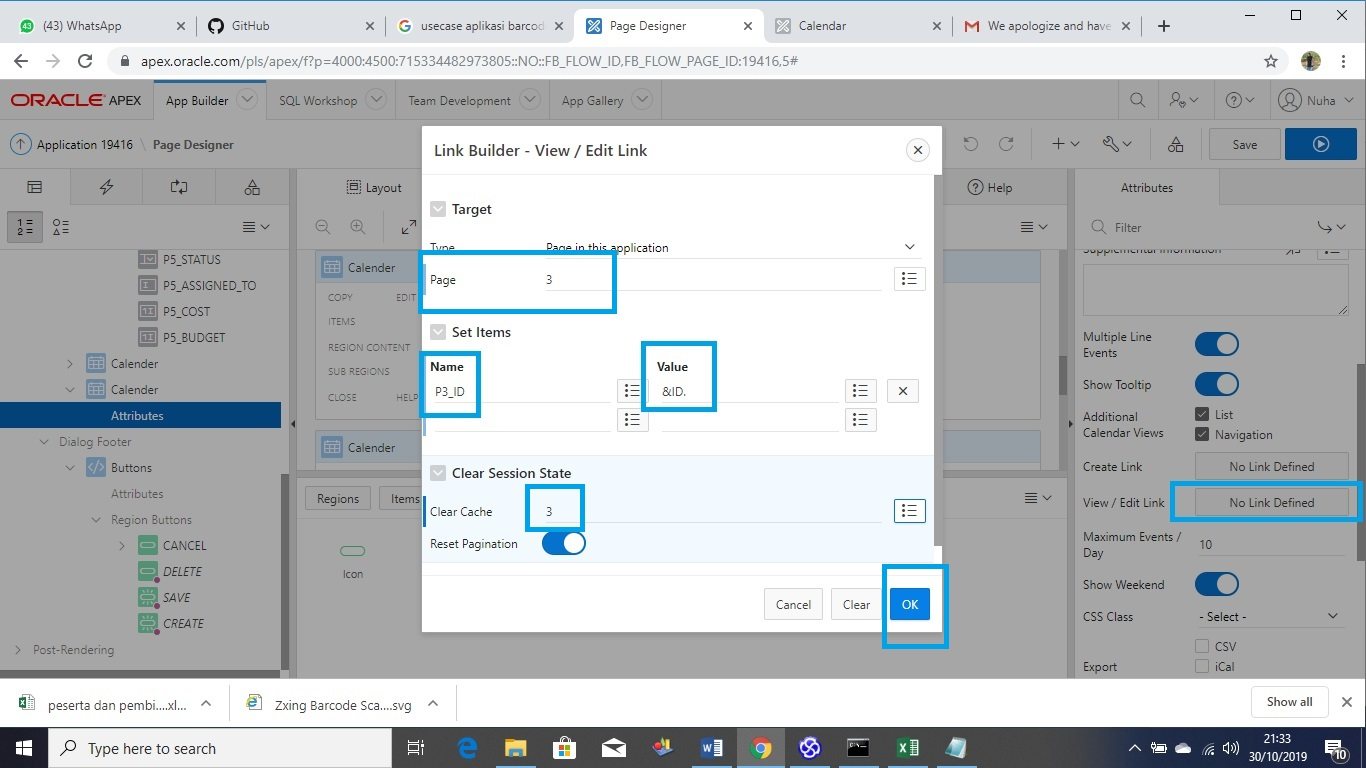
\includegraphics[width=11cm\textwidth]{calender5.jpg}
    \end{center}
    \item Klik Save and Run pada kanan atas
    seharusnya:
     \begin{center}
    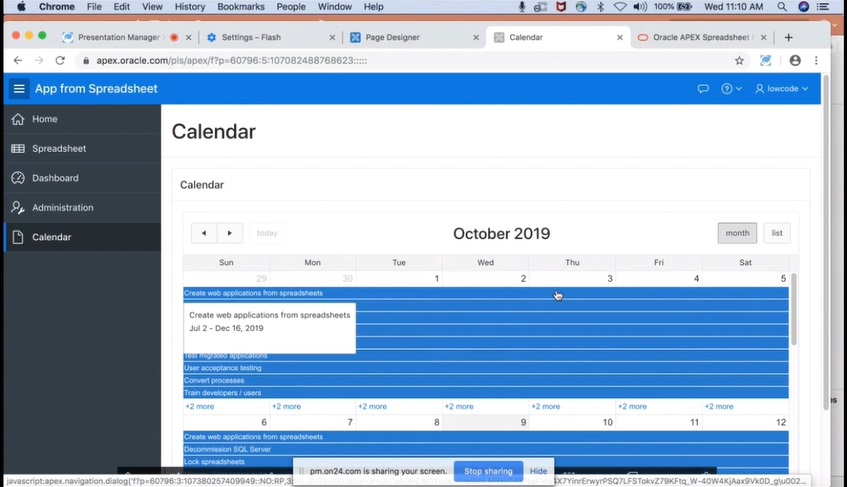
\includegraphics[width=11cm\textwidth]{calendeeer.jpg}
    \end{center}
    tapi karena ada kesalahan seperti ini
      \begin{center}
    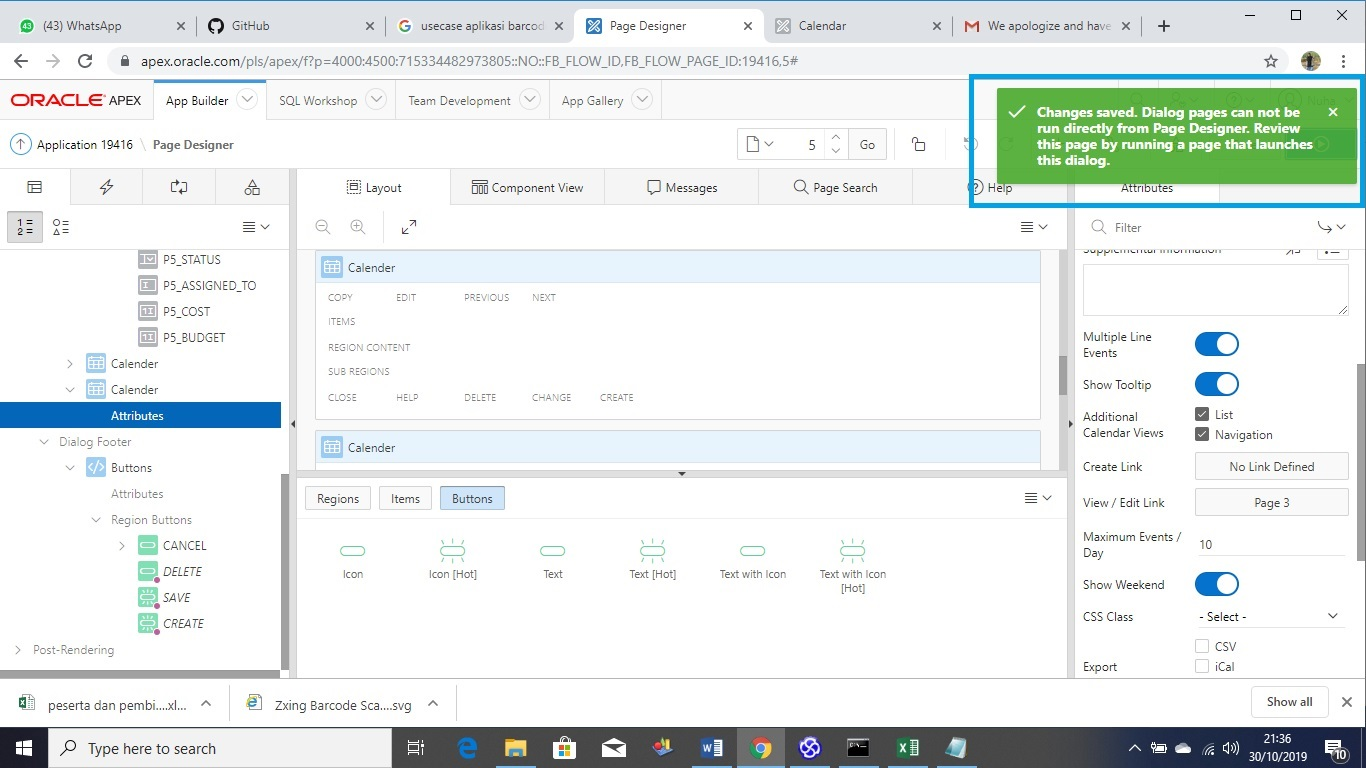
\includegraphics[width=11cm\textwidth]{calendereror.jpg}
    \end{center}
\end{enumerate}

\end{document}
